\documentclass[openany]{book}
\usepackage[utf8]{inputenc}
\usepackage[T1]{fontenc}
\usepackage[spanish]{babel}
\usepackage{geometry}
\usepackage{graphicx}
\usepackage{natbib}
\usepackage{multirow}
\usepackage{booktabs}
\usepackage{algorithmic}
\usepackage{algorithm}
\usepackage{setspace}
\usepackage{pdfpages}
\usepackage[toc,page]{appendix}
\RequirePackage{amsfonts,amsmath,amssymb,amsthm}
\newgeometry{top=3cm,bottom=3cm,left=3cm,right=3cm}

\newcommand*\Bell{\ensuremath{\boldsymbol\ell}}
\renewcommand{\appendixtocname}{Ap\'endices}
\renewcommand{\appendixpagename}{Ap\'endices}
\addto\captionsspanish{\renewcommand\chaptername{Secci\'on}}

\begin{document}
\frontmatter
\thispagestyle{empty}

\begin{flushright}
	\includegraphics[scale=0.2]{fig/logo_unl.png}
\end{flushright}
\vskip-2.5cm %\noindent
\textrm{ UNIVERSIDAD NACIONAL DEL LITORAL}

\vspace{2cm}

\begin{center}
	\noindent \textrm{\large DOCTORADO EN INGENIERÍA}
\end{center}

\vspace{2.5cm}


\noindent\textrm{\bf \huge Nuevo enfoque de aprendizaje}\\[0.2 cm]
\noindent\textrm{\bf \huge semi-supervisado para la identificación} \\[0.2 cm]
\noindent\textrm{\bf \huge de secuencias en bioinformática}

\vspace{1.5cm}

\noindent \textrm{{\LARGE Cristian Ariel Yones}}

\vspace{3cm}


\noindent \textrm{FICH} \\
\noindent \textrm{\small FACULTAD DE INGENIERÍA}\\
\noindent \textrm{\small Y CIENCIAS HÍDRICAS}
\vspace{0.4cm}

\noindent \textrm{sinc(\textit{i})}\\
\noindent \textrm{\small INSTITUTO DE INVESTIGACIÓN EN SEÑALES}\\
\noindent \textrm{\small SISTEMAS E INTELIGENCIA COMPUTACIONAL}
\vspace{0.4cm}

\noindent \textrm{INTEC}\\
\noindent \textrm{\small INSTITUTO DE DESARROLLO TECNOLÓGICO}\\
\noindent \textrm{\small PARA LA INDUSTRIA QUÍMICA}
\vspace{0.4cm}

\noindent \textrm{CIMEC}\\
\noindent \textrm{\small CENTRO DE INVESTIGACIÓN DE}\\
\noindent \textrm{\small MÉTODOS COMPUTACIONALES}


\vspace{1cm}

\begin{flushright}
	\noindent \large{Tesis de Doctorado \textbf{2018}}
\end{flushright}


\newpage
\thispagestyle{empty}
\begin{center}

	\includegraphics[scale=.2]{fig/logo_unl.png}

{\large UNIVERSIDAD NACIONAL DEL LITORAL}\\
{Facultad de Ingeniería y Ciencias Hídricas\\
Instituto de Investigación en Señales, Sistemas e Inteligencia Computacional}
\vspace{3.5cm}

\textbf{\Large NUEVO ENFOQUE DE APRENDIZAJE}\\[0.1 cm]
\textbf{\Large SEMI-SUPERVISADO PARA}\\[0.1 cm]
\textbf{\Large LA IDENTIFICACIÓN DE}\\[0.1 cm]
\textbf{\Large SECUENCIAS EN BIOINFORMÁTICA}\\[0.1 cm]

\vspace{1cm}

\textbf{\large Cristian Ariel Yones}

\vspace{4cm}

\small Tesis remitida al Comité Académico del Doctorado como \\[0.01 cm]
\small parte de los requisitos para la obtención del grado de \\[0.01 cm]
\small DOCTOR EN INGENIERÍA                                 \\[0.01 cm]
\small Mención en Inteligencia Computacional, Señales y Sistemas        \\[0.1 cm]
\small de la                                                \\[0.01 cm]
\small UNIVERSIDAD NACIONAL DEL LITORAL                     \\[0.5 cm]

\textbf{\large 2018}

\vspace{1.8cm}

{\footnotesize Comisión de Posgrado, Facultad de Ingeniería
y Ciencias Hídricas, Ciudad Universitaria, Paraje ``El Pozo'',
S3000, Santa Fe, Argentina.}

\end{center}

\restoregeometry

\newgeometry{top=3cm,bottom=2cm,left=3cm,right=3cm}
\thispagestyle{empty}

\begin {center}

\includegraphics[scale=.25]{fig/logo_unl.png}

{\large UNIVERSIDAD NACIONAL DEL LITORAL}\\
{Facultad de Ingeniería y Ciencias Hídricas\\Instituto de Investigación en Señales, Sistemas e Inteligencia Computacional}

\vspace{3cm}
\textbf{\Large NUEVO ENFOQUE DE APRENDIZAJE}\\[0.1 cm]
\textbf{\Large SEMI-SUPERVISADO PARA}\\[0.1 cm]
\textbf{\Large LA IDENTIFICACIÓN DE}\\[0.1 cm]
\textbf{\Large SECUENCIAS EN BIOINFORMÁTICA}\\[0.1 cm]
\vspace{1cm}

\textbf{\large Cristian Ariel Yones}\\

\vspace{1cm}

\end{center}

{\large \noindent \textbf{Lugar de Trabajo:}\\
\vspace{1em}sinc(i)\\
Instituto de Señales, Sistemas e Inteligencia Computacional\\
Facultad de Ingeniería y Ciencias Hídricas\\
Universidad Nacional del Litoral\\[0.5cm]

\noindent\textbf{Director:}\\
Dr. Diego H. Milone\hspace{13.2em} sinc(\textit{i}), CONICET-UNL\\[0.4cm]
\noindent\textbf{Co-director:}\\
Dra. Georgina Stegmayer\hspace{11em} sinc(\textit{i}), CONICET-UNL\\[0.4cm]

\noindent\textbf{Jurado Evaluador:}\\[0.3cm]
Dr. Pablo Manavella\hspace{13.1em} IAL, CONICET-UNL\\[0.1cm]
Dr. Guillermo Grinblat\hspace{12em} CIFASIS, CONICET-UNR\\[0.1cm]
Dr. Carlos Chesñevar\hspace{12.8em} ICIC, CONICET-UNS\\[0.1cm]
Dra. Jéssica Carballido\hspace{12.1em} ICIC, CONICET-UNS\\[0.1cm]
}

\newpage
\thispagestyle{empty}
\vspace*{3em}
{\hfill\large \textbf{DECLARACIÓN LEGAL DEL AUTOR}\hfill\mbox{}}
\vspace{1em}

Esta Tesis ha sido remitida como parte de los requisitos para la obtención del grado académico de Doctor en Ingeniería ante la Universidad Nacional del Litoral
y ha sido depositada en la Biblioteca de la Facultad de Ingeniería y Ciencias Hídricas para que esté a disposición de sus lectores bajo las condiciones
estipuladas por el reglamento de la mencionada Biblioteca.

Se permiten citaciones breves de esta Tesis sin la necesidad de un permiso especial, en la suposición de que la fuente sea correctamente citada. El portador
legal del derecho concedera por escrito solicitudes de permiso para la citación extendida o para la reproducción parcial o total de ese manuscrito serán
concebidos por el portador legal del derecho de propiedad intelectual de la obra, por medio escrito.

\newpage
\thispagestyle{empty}
\vspace*{3em}
{\hfill\large \textbf{TESIS POR COMPILACIÓN}\hfill\mbox{}}
\vspace{1em}

La presente tesis se encuentra organizada bajo el formato de Tesis por Compilación,
aprobado en la resolución No 255/17 (Expte. No 888317-17) por el Comité Académico
de la Carrera Doctorado en Ingeniería, Facultad de Ingeniería y Ciencias Hídricas,
Universidad Nacional del Litoral (UNL). De dicha resolución:

``En el caso de optar por la Tesis por Compilación, ésta consistirá en una descripción
técnica de al menos 30 páginas, redactada en español e incluyendo todas las investi-
gaciones abordadas en la tesis. Se deberán incluir las secciones habituales indicadas
a continuación en la Sección Contenidos de la Tesis. Los artículos científicos publi-
cados por el autor, en el idioma original de las publicaciones, deberán incluirse en
un Anexo con el formato unificado al estilo general de la Tesis indicado en la Sección
Formato. El Anexo deberá estar encabezado por una sección donde el tesista detalle
para cada una de las publicaciones cuál ha sido su contribución. Esta sección deberá
estar avalada por su director de Tesis. El documento central de la Tesis debe incluir
referencias explícitas a todas las publicaciones anexadas y presentar una conclusión
que muestre la coherencia de dichos trabajos con el hilo conceptual y metodológico
de la tesis. Los artículos presentados en los anexos podrán ser artículos publicados,
aceptados para publicación (en prensa) o en revisión.''


\tableofcontents

\renewcommand{\listtablename}{\'Indice de tablas}

\listoftables
\listoffigures

\newpage
\thispagestyle{empty}

\vspace{3cm}
\begin{center}
{\huge \textbf{Resumen}}
\end{center}
\vspace{1cm}

Los microARN (miARN) son un grupo de pequeñas secuencias de ácido ribonucleico (ARN) no codificante que desempeñan un papel muy importante en la
regulación génica. En los últimos años, se han desarrollado una gran cantidad de métodos que intentan detectar nuevos miARNs utilizando sólo información
secuencial, es decir, sin medir niveles de expresión. El primer paso en estos métodos generalmente consiste en extraer del genoma subcadenas que cumplan con
ciertos requerimientos estructurales. En segundo lugar se extraen características numéricas de estas subcadenas para finalmente usar aprendizaje maquinal
para predecir cuáles probablemente contengan miARN. Existen varias deficiencias en las metodologías propuestas. En primer lugar, muy poco se ha tratado el
problema de la extracción de subcadenas del genoma completo. Este paso normalmente desatendido es muy importante ya que: i) los miARNs que se pierdan en esta
etapa no se podrán recuperar en etapas posteriores y ii) definir correctamente los límites de las subcadenas extraídas es muy importante para que los
algoritmos de aprendizaje maquinal generen predicciones correctas. Por otro lado, en paralelo con los métodos de predicción de miARN se han propuesto una gran
cantidad de características para representar numéricamente las subcadenas de ARN. Algunas de estas características se pueden calcular con distintas
herramientas, pero estas se desarrollaron con distintos lenguajes de programación y presentan interfaces muy variadas (línea de comandos, web, etc.). Para
algunas características directamente no se cuenta con herramientas de acceso libre. Finalmente, la mayoría de los métodos actuales usan aprendizaje
supervisado para la etapa de predicción. Este tipo de métodos tienen importantes limitaciones prácticas cuando deben aplicarse a tareas de predicción real.
Existe el desafío de lidiar con un número escaso de ejemplos de pre-miARN positivos. Además, es muy difícil construir un buen conjunto de
ejemplos negativos para representar el espectro completo de secuencias no miARN. Por otro lado, en cualquier genoma, existe un enorme desequilibrio de clase
($1:10000$) que es bien conocido por afectar particularmente a los clasificadores supervisados.

Para permitir predicciones precisas y rápidas de nuevos miARNs en genomas completos, en esta tesis se realizaron aportas en las tres etapas del proceso de predicción de miARN.
En primer lugar, se desarrollo una metodología para extraer subcadenas del genomas completo que cumplan con los requerimientos mínimos para ser candidatas a
miARN. En segundo lugar, se desarrollo una herramienta que permite calcular la mayoría de las características utilizadas para predicciones de miARN en el estado
del arte. La tercer contribución consiste en un algoritmo novedoso de aprendizaje maquinal semi-supervisado que permite realizar predicciones a partir de muy pocos
ejemplos. Este tipo de aprendizaje aprovecha la información provista por las subcadenas desconocidas (sobre las que se desea generar predicciones)
para mejorar las tasas de predicción. Esta información extra permite atenuar el efecto del número reducido de ejemplos etiquetados y la pobre
representatividad de las clases.

Se comparó el método propuesto de extracción de secuencias tipo horquilla con el único método disponible para tal tarea en la actualidad en 6 especies y se obtuvo
en todos los casos mejores resultados, tanto en cantidad de horquillas como en cantidad de pre-miARNs conocidos encontrados. Se realizaron pruebas para validar los
algoritmos de extracción de características, obteniendo resultados correctos en todos los casos. Finalmente, se realizaron pruebas del método de aprendizaje maquinal
propuesto con datos genómicos de tres especies modelo, con más de un millón de subcadenas cada una. Se hicieron comparaciones con una gran cantidad de métodos del estado del arte,
obteniéndose mejores tasas de predicción y tiempos de ejecución más cortos.


\mainmatter

\chapter{Introducción}
\section{Aprendizaje automático semi-supervisado}

El aprendizaje automático es un campo de las ciencias de la computación que intenta dotar a los sistemas informáticos de la capacidad de aumentar
progresivamente su habilidad en una tarea específica, sin la necesidad de ser específicamente programados para tal tarea \citep{samuel1959some}. Dentro de este
campo podemos identificar dos grandes grupos de técnicas: las de aprendizaje supervisado y las de aprendizaje no supervisado. Las primeras utilizan un conjunto
de datos que traen asociados una etiqueta de clase (que indica a qué clase pertenece el objeto) o valor de salida deseado. El proceso de aprendizaje consiste en
generar un modelo que logre mapear los datos de entrada a los valores de salida deseados \citep{russell2016artificial}. El modelo además debe ser capaz de
generalizar, es decir, generar salidas correctas cuando reciba como entrada datos no vistos durante el proceso de aprendizaje. Por otro lado, en el aprendizaje
no supervisado el objetivo es generar modelos que descubran grupos o relaciones subyacentes en los datos sin utilizar ningún tipo de etiqueta o valor de salida
esperado.

Como punto intermedio entre los dos grupos de técnicas antes mencionados, apareció un nuevo grupo de algoritmos, llamados de aprendizaje
semi-supervisado \citep{chapelle2006semi}. Este tipo de algoritmos utiliza ejemplos etiquetados para aprender la distribución de las clases de la misma forma
que los métodos de aprendizaje supervisado, pero además aprovecha ejemplos no etiquetados para modelar mejor el espacio de las características y así mejorar las
tasas de clasificación. Como los ejemplos no etiquetados proveen información extra sobre la distribución de los datos en el espacio de las características, este
grupo de técnicas obtiene buenas tasas de clasificación en problemas donde la cantidad de datos etiquetados es baja o no es representativa de su clase.  En la
Figura~\ref{fig:semivssuperv} podemos ver un ejemplo muy simple de cómo datos sin etiqueta pueden ayudar a reconocer los límites de las clases de interés.
En~\ref{fig:semivssuperv}.a vemos 4 ejemplos de entrenamiento de dos clases diferentes y la frontera de decisión que construiría un clasificador supervisado con
estos datos de entrada. En el siguiente cuadro vemos que los datos de entrenamiento en realidad no eran representativos de sus clases por lo que la frontera de
decisión falla al separarlas. Por otro lado, si se utiliza un esquema semi-supervisado (~\ref{fig:semivssuperv}.c) este aprovecha tanto los datos etiquetados
como los no etiquetados para descubrir la distribución latente de los datos y de esta forma separar las dos clases satisfactoriamente.

% Durante la última década, una gran parte de las técnicas que se han desarrollado en el campo del aprendizaje semi-supervisado utiliza representaciones de los
% datos en forma de grafos. Estas técnicas representan cada dato como un nodo del grafo y una arista conecta dos nodos si son de alguna manera similares.  Luego,
% utilizando los nodos etiquetados, se predicen etiquetas para el resto de los nodos. Estos métodos han mostrado buenas tasas de desempeño
% \citep{joachims2003transductive} y además son algoritmos muy escalables que, correctamente implementados, permiten el manejo de grandes volúmenes de datos.

Un concepto que está estrechamente relacionado con el aprendizaje semi-supervisado es el de aprendizaje transductivo. En esta configuración, los datos de
entrenamiento se utilizan para hacer directamente inferencias en datos de prueba. A diferencia de la mayoría de los métodos inductivos, donde el algoritmo
tiene dos etapas (entrenamiento e inferencia), los métodos transductivos tienen sólo una etapa, como se muestra en la figura ~\ref{fig:schemes}. En el esquema
inductivo (a), el algoritmo de aprendizaje utiliza datos de entrenamiento etiquetados para ajustar un modelo. En la segunda etapa, el modelo ya ajustado se usa
para hacer predicciones sobre datos nuevos (no vistos durante el entrenamiento). En el esquema transductivo (b), tanto los datos etiquetados como los no
etiquetados se procesan juntos, en la misma etapa. Como resultado, se obtienen etiquetas para los datos no etiquetados, pero ninguna función de decisión, modelo
entrenado o regla de clasificación. Cabe señalar que la validación de cualquier método de transducción es bastante diferente de una estándar (inductiva). Dado
que el entrenamiento y la predicción se combinan en una etapa, al algoritmo se le proporcionan tanto los datos de entrenamiento como los de prueba, pero los
segundos sin etiquetas. Este tipo especial de validación se utiliza en todos los algoritmos transductivos \citep{chapelle2006semi}, donde las etiquetas de los
casos de prueba nunca se utilizan en ningún paso de la etapa de predicción.

\begin{figure}[tpb]
	\centering
	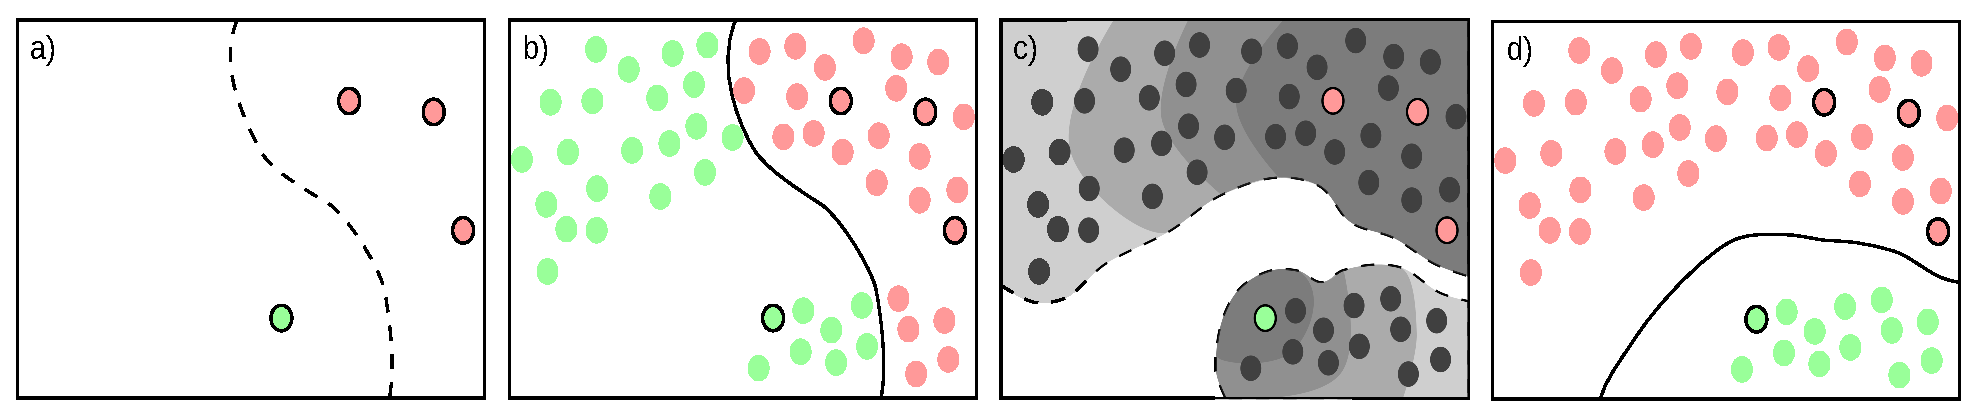
\includegraphics[width=\textwidth]{fig/semivssuperv.eps}
	\caption[Aprendizaje semi-supervisado vs supervisado]{Ejemplo de clasificación con aprendizaje supervisado (a-b) y con aprendizaje semi-supervisado (c-d).}
	\label{fig:semivssuperv}
\end{figure}

\section{Predicción automática de microARN}

En los últimos años, la biología molecular demostró un importante avance en distintas áreas de la investigación. Esta disciplina científica
estudia la estructura, función y composición de las moléculas biológicamente importantes y se relaciona fuertemente con otras áreas como la
genética y la bioquímica. En la actualidad se invierte un gran esfuerzo en estudiar las interacciones entre los numerosos sistemas de las células,
incluyendo las interacciones entre los diferentes tipos de ácido desoxirribonucleico (ADN), ácido ribonucleico (ARN) y los procesos de síntesis de
proteínas, y también cómo estas interacciones son reguladas. Los avances en este campo permiten la generación de una gran cantidad de información
que requiere el uso de herramientas de cálculo altamente especializadas para el análisis. En este contexto, la bioinformática ha tomado un papel muy
importante ya que aporta herramientas que posibilitan la explotación de estos datos.

Un problema abierto en Bioinformática desde hace más de una década es el de la predicción automática de microARNs (miARNs). Los miARNs son una clase de
pequeñas moléculas ($\sim$21 nucleótidos) monocatenarias de ácido desoxirribonucleico no codificante que regulan la expresión de otros genes. Se
encuentran presentes tanto en animales como en plantas y su importancia en procesos biológicos clave ha sido ampliamente documentada
\citep{rosenzvit2013microrna}. Los miARNs están implicados, por ejemplo, en la evolución del cáncer (sea como inhibidores o promotores de éste)
\citep{yu2015microrna}, en procesos de infección viral \citep{lecellier2005}. Además, identificar los microARNs de ciertas especies tiene aplicaciones
directas, como puede en plantas ser la mejora de cultivos \citep{liu2010new} o, en animales,  el desarrollo de nuevas vacunas y antibióticos
\citep{tsetsarkin2017synergistic}. Estas pequeñas moléculas normalmente se transcriben a partir de secuencias primarias de mayor tamaño, llamadas
pri-miARNs. Durante la biogénesis, las secuencias precursoras se pliegan sobre sí mismas formando una estructura secundaria tipo tallo-horquilla como se
puede ver en la Figura~\ref{fig:mirna}. Luego son separadas de la secuencia principal y trasladadas fuera del núcleo. En este paso, la estructura toma el
nombre de precursora del miARN o pre-miARN. Finalmente el miARN es liberado del precursor para tomar un papel activo en la regulación de la expresión de los
genes.

\begin{figure}[tpb]
	\centering
	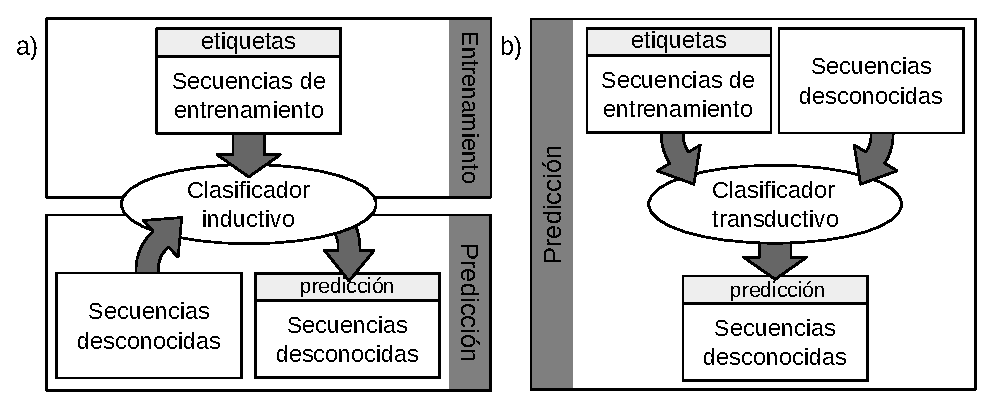
\includegraphics[width=\textwidth]{fig/paradigmas.eps}
	\caption[Aprendizaje inductivo vs. transductivo]{Aprendizaje inductivo y transductivo. a) Esquema tradicional inductivo con dos etapas separadas; b)
	Esquema transductivo con sólo una etapa.}
	\label{fig:schemes}
\end{figure}

En la última década, se utilizaron numerosos enfoques experimentales y computacionales para identificar nuevos miARNs. Los métodos experimentales que se han
usado tradicionalmente como el clonado directo son capaces de detectar sólo miARNs que se expresan de forma abundante \citep{kleftogiannis2013where}. Los
últimos avances en secuenciación permiten un alto nivel de cobertura, mitigando estos efectos \citep{an2013mirdeep}. Sin embargo, aquellos que se expresan en
ciertas etapas de una especie, o en tejidos específicos, pueden no ser detectados. Por otro lado, el desarrollo y posterior análisis de los modelos
computacionales entrenados para reconocer miARNs puede brindar pistas que permitan caracterizar mejor estas moléculas y su biogénesis. Los enfoques
computacionales utilizados para la clasificación de secuencais candidatas a miARN pueden dividirse en dos grupos: métodos por homología y métodos de aprendizaje
automático. Los primeros se basan en la conservación de miARNs entre especies estrechamente relacionadas y, por lo tanto, no pueden usarse para miARNs que son
específicos de una especie \citep{ng2007novo}. Los métodos de aprendizaje automático utilizan un enfoque diferente, que consiste en extraer primero
características de pre-miARNs conocidos, de secuencias que se utilizarán como ejemplos negativos y de las secuencias desconocidas que se desea clasificar.
Después se utilizan las características de las secuencias conocidas (tanto positivas como negativas) para entrenar un clasificador de forma supervisada, para
finalmente aplicarlo a las secuencias no conocidas y obtener una predicción \citep{kleftogiannis2013where}. Las características que pueden usarse para
representar secuencias de ARN han sido ampliamente estudiadas \citep{Lopes2014}. Además, muchos algoritmos de aprendizaje supervisado han sido aplicados a este
problema: máquinas de soporte vectorial, modelos ocultos de Markov y ensambles de clasificadores, entre otros \citep{kleftogiannis2013where}. Sin embargo
todavía existen muchos problemas abiertos en la predicción de pre-miARNs con técnicas de aprendizaje maquinal \citep{stegmayer2018predicting}.

La gran mayoría de los métodos de predicción del estado del arte toman como entrada secuencias con estructura secundaria tipo tallo-horquilla y se encargan
luego de extraer características, entrenar un clasificador y hacer predicciones. Si bien este primer paso generalmente es ignorado, es fundamental para lograr
buenos resultados en las etapas posteriores. No sólo es importante lograr capturar todas las secuencias con estructura secundaria tipo tallo horquilla del
genoma, sino que también es fundamental que estas secuencias se corten en los lugares correctos. Si un pre-miARN se corta erróneamente con una longitud mayor
o menor a la real, las características calculadas pueden variar mucho y generar resultados erróneos durante la etapa de predicción. Actualmente, la única
herramienta disponible para esta tarea \citep{durbin1999einverted} no aprovecha los últimos avances en cuanto a la estimación de estructuras secundarias, por
lo que el número de secuencias que detecta es bajo y muchos pre-miARN se pierden durante esta temprana etapa. Además, no se tiene en cuenta el contexto de la
secuencia para detectar dónde son los mejores puntos de corte. Las características utilizadas en la predicción de pre-miARN son muy sensibles a pequeñas
diferencias en el corte, por lo que elegir el punto óptimo es crucial para obtener buenos resultados en la clasificación.

Por otro lado, durante la última década se ha desarrollado una gran cantidad de características específicamente para el problema de predicción de
microARN, que se pueden extraer tanto de las secuencias o sus estructuras secundarias. Se han publicado muchas herramientas para calcular algunas de estas
características, pero estas están codificadas en diferentes lenguajes de programación y tienen diferentes modos de acceso (web, línea de comandos, etc.).
Además, varias de estas herramientas son software propietario y el código fuente no está disponible \footnote{http://www.insybio.com/pages/ncrnaseq}. Estas
cuestiones dificultan en gran medida el uso de muchas de estas características.

\begin{figure}[t]
	\centering
	\includegraphics[width=\textwidth]{fig/mirna.pdf}
	\caption[Estructura secundaria de un pre-miARN]{Estructura secundaria de un pre-miARN humano. En rojo se puede ver resaltado el miARN hsa-let-7e.}
	\label{fig:mirna}
\end{figure}

Por último, la etapa de predicción o clasificación de secuencias como posibles candidatos a pre-miARN aún presenta importantes dificultades que no han sido
resueltas satisfactoriamente. En primer lugar, aunque el número de secuencias no pre-miARN que se pueden encontrar en cualquier genoma es grande, los ejemplos
negativos que se utilicen deben ser representativos de la gran variedad de secuencias no pre-miARN. Un estudio \citep{wei2014improved} analizó la
importancia de los ejemplos negativos utilizados y cómo esto limita el rendimiento de los clasificadores. En la mayoría de los casos, los conjuntos negativos
que se usan para ajustar los modelos de clasificación se definen principalmente con secuencias tomadas de regiones de codificación de proteínas, ARNm u otras
regiones donde es poco probable encontrar miARN \citep{peace2015framework, tempel2015mirboost}. Nada puede asegurar que estas secuencias sean buenos
representantes de todas las posibles secuencias no pre-miARN, o que estén lo suficientemente cerca de los límites de la verdadera clase de pre-miARN. Por ejemplo,
si el poder de predicción de un clasificador se prueba en un conjunto de datos que tiene pre-miARNs y ncARNs, lo que realmente se está midiendo es la capacidad
de diferenciar entre estos dos tipos de secuencia, pero el clasificador podría no descartar correctamente otras secuencias no pre-miARN. Ningún método ha
informado tasas de error teniendo en cuenta este punto crucial. Para abordar este problema, algunos métodos utilizan secuencias tomadas de posiciones aleatorias
de un genoma como ejemplos negativos \citep{wenyuan2013training, gudys2013huntmi}. Sin embargo, en este caso, nada puede garantizar que un pre-miARN no conocido
se utilice erróneamente como un ejemplo negativo. En ambas estrategias de construcción de conjuntos de ejemplos negativos, no se puede garantizar que los
ejemplos sean representativos de toda la clase negativa; y, lo que es peor, algunos de ellos podrían ser falsos negativos. Otra característica de este problema
que dificulta la aplicación simple de técnicas de aprendizaje maquinal es el hecho de que el número de ejemplos positivos es muy bajo en cualquier genoma, por
lo cual este constituye un problema con muy alto desbalance entre clases. Este problema es aún peor en especies no modelo, donde la cantidad de secuencias
anotadas es menor. Una alternativa puede ser utilizar pre-miARNs de especies cercanas como ejemplos positivos, pero recientemente se ha demostrado
\citep{lopes2016automatic} que el problema de predicción de pre-miARNs es muy dependiente de la especie, por lo que esta estrategia puede afectar el desempeño
de las técnicas de predicción. Por otro lado, la gran variedad de secuencias que se pueden utilizar como ejemplos negativos y el bajo número de ejemplos
positivos obliga a entrenar clasificadores con un desbalance muy grande entre el número de secuencias positivas y las potencialmente negativas. Esto presenta
una dificultad adicional ya que está demostrado que las  técnicas estándar de aprendizaje maquinal son muy sensibles al desbalance de clases
\citep{guo2008class}.


\chapter{Objetivos}
\section{Objetivo general}

El objetivo general de esta tesis es desarrollar nuevos métodos para la clasificación de candidatos a pre-miARN a partir del  genoma completo tanto de
animales como de plantas, y capaces de desempeñarse adecuadamente en un contexto de gran desbalance entre la clase de interés y una alta proporción de
secuencias no etiquetadas.

\section{Objetivos específicos}

A continuación se detallan los objetivos específicos de la presente investigación:
\begin{itemize}
	\item Revisar e integrar todas las características utilizadas en la actualidad para la predicción de pre-miARNs.
	\item Desarrollar una metodología integrada y simple que permita encontrar automáticamente secuencias tipo tallo-horquilla en genomas completos.
	\item Desarrollar nuevos algoritmos de clasificación que incorporen etapas de aprendizaje semi-supervisado para atacar los problemas de gran
		desbalance de clases y alta proporción de ejemplos no etiquetados.
	\item Validar las propuestas con genomas reales a través del trabajo multidisciplinario con expertos del dominio.
\end{itemize}


\chapter{Métodos propuestos}
Siguiendo las ideas presentadas previamente, en la Figura 2 se presenta la metodología general diseñada para la clasificación y predicción de nuevos
microARNs. La metodología o proceso consiste en tres etapas, en primer lugar se deben extraer todas las subcadenas del genoma que tengan una estructura
secundaria similar a la de un pre-miARN. Luego, a estas secuencias candidatas se les extraen características para convertirlas en vectores numéricos,
procesables con métodos de aprendizaje maquinal. En paralelo, se comparan todas las subcadenas con los pre-miARNs de conocidos (tomados de la base de datos mirBase)
para marcar los ejemplos positivos. Finalmente, se obtienen predicciones para las secuencias no etiquetadas utilizando un algoritmo de aprendizaje maquinal
semi-supervisado. En las siguientes subsecciones se describe con más detalle cada etapa del proceso.

\section{Procesamiento de secuencias de ARN de tipo tallo-horquilla}
Como se mencionó antes, los pre-miARNs se pliegan en estructuras secundarias tipo tallo- horquilla. Estas secuencias tienen una longitud promedio que depende
de la especie, y un nivel de emparejamiento relativamente alto. Estas características especiales de los pre-miARNs, además de ser útiles para una primer
etapa de filtrado, se pueden utilizar para cortar el genoma completo en subcadenas que pueden ser procesadas más fácilmente por las siguientes etapas. El
objetivo de esta etapa es entonces extraer todas las secuencias tipo tallo-horquilla de un genoma cortando en los puntos donde se obtienen las estructuras
secundarias con la mayor estabilidad termodinámica posible. Para ello se sigue el esquema de pasos presentado en la Figura~\ref{fig:hextractor}. A
continuación se detalla cada paso de este proceso:

\begin{figure}[h]
	\centering
	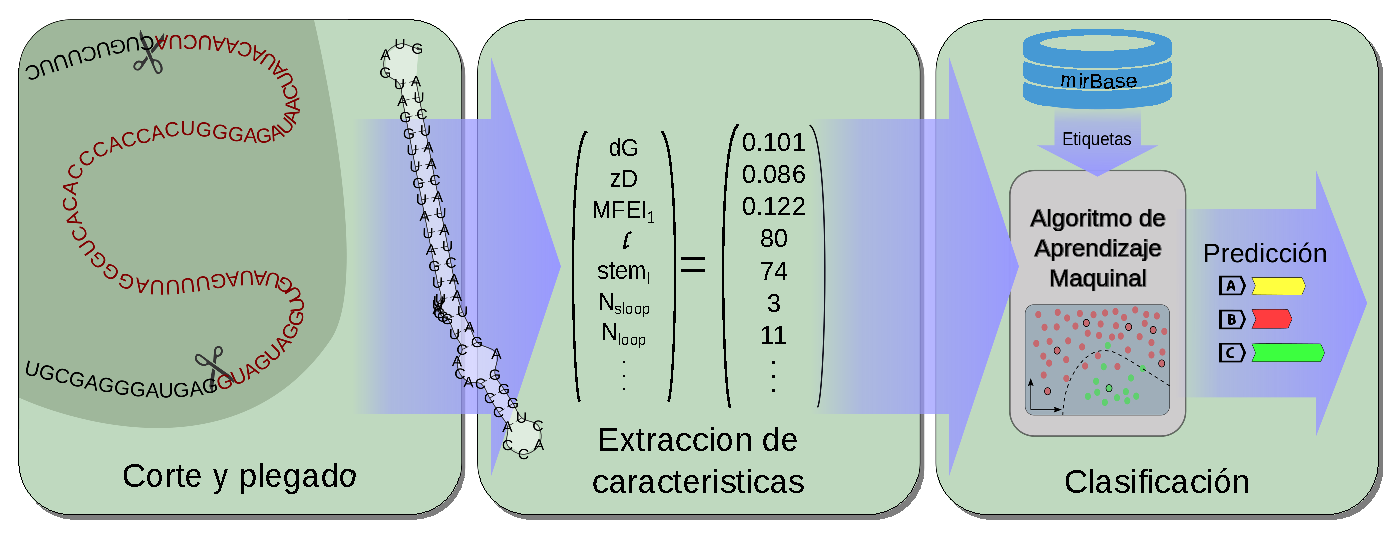
\includegraphics[width=\textwidth]{fig/diagrama.eps}
	\caption[Etapas de la predicción de microARN]{proceso completo de predicción de nuevos pre-miARNs, separado en sus tres etapas principales.}
	\label{fig:esquema}
\end{figure}

\subsection{Ventaneo del genoma}

Se comienza cortando el genoma completo en ventanas solapadas de una longitud varias veces mayor (~500 nt.) a la de un pre-miARN promedio. La ventana debe ser
lo suficientemente larga para poder capturar la horquilla completa pero además para que se tenga en cuenta el entorno de cualquier posible horquilla al
estimar la estructura secundaria. Esto último es muy importante ya que los resultados de estimar la estructura secundaria se ven muy afectados por el entorno
de la secuencia. Por ejemplo, sin considerar el entorno de una secuencia, la estructura secundaria estimada puede presentar una estabilidad menor a la que se
formaría si se habría considerado el entorno.

\subsection{Plegado y poda}

\begin{figure}[t]
	\centering
	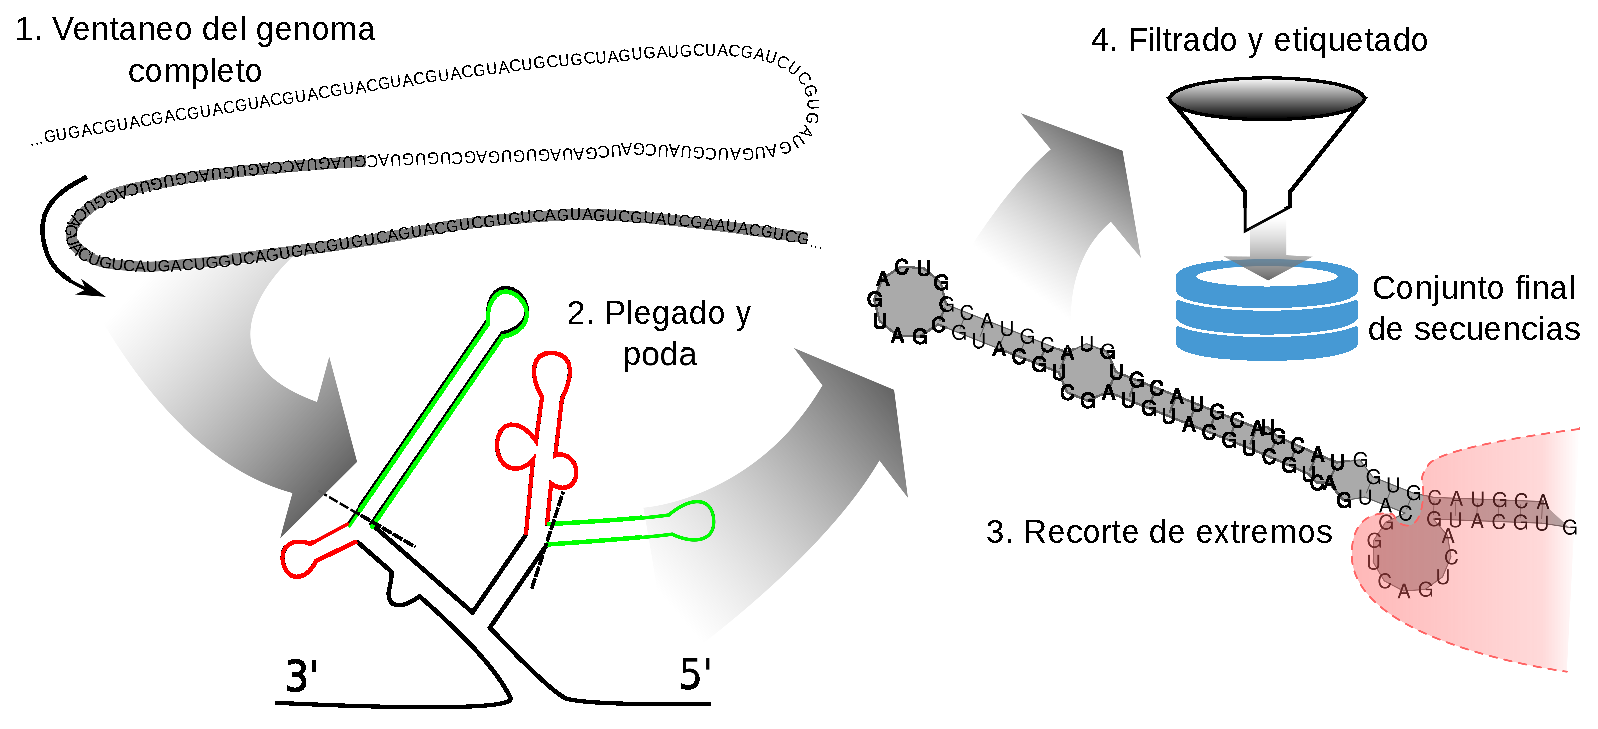
\includegraphics[width=\textwidth]{fig/hextractor.eps}
	\caption[Extracción de secuencias tipo tallo-horquilla]{proceso de extracción de secuencias tipo tallo-horquilla del genoma completo.}
	\label{fig:hextractor}
\end{figure}

Se predice la estructura secundaria que formaría cada una de las ventanas al plegarse. Para ello se utiliza el algoritmo de mínima energía libre
\citep{zuker1981optimal}. Este algoritmo utiliza programación dinámica para encontrar la estructura secundaria que minimiza la energía liberada. Dado que
las ventanas utilizadas son relativamente largas, las estructuras normalmente presentan múltiples bucles. Por lo tanto, el siguiente paso es buscar los puntos
de corte que logren separar la estructura completa en varias estructuras tipo horquilla, como se puede ver en la Figura~\ref{fig:hextractor}. De las horquillas
extraídas, se eliminan las que no superan una longitud y nivel de emparejamiento mínimo y el resto pasa a la siguiente etapa.

\subsection{Recorte de secuencias}

Como se utilizaron ventanas de una longitud varias veces mayor a la de un pre-miARN promedio, generalmente las secuencias encontradas forman estructuras
secundarias mayores a la de un pre-miARN. Por este motivo es importante analizar cada secuencia para detectar si es necesario un recorte. Como aún se
desconoce el funcionamiento de las enzimas que se encargan de separar el pre-miARN de la secuencia, se utilizan ciertas heurísticas que permiten obtener
secuencias con longitudes y estabilidad similares a las de un pre-miARN. Estas reglas intentan optimizar la Mínima Energía Libre Normalizada (NMFE, por
sus siglas en ingles \textit{Normalized Minimum Free Energy}), que se sabe es muy baja en las estructuras secundarias de los pre-miARNs, respetando ciertos
límites en la longitud de la secuencia. La NMFE es la energía termodinámica que libera la secuencia al plegarse, por lo tanto, cuanto mayor es la energía
que se libera más estable es la estructura secundaria.

Si bien se podrían encontrar de forma óptima los puntos de corte óptimo, re-estimando la estructura secundaria para todos los cortes posibles, se decidió
utilizar un conjunto de reglas que aproximan esta solución. De esta forma, además de acelerar en gran medida el procesamiento, se logra una mayor
flexibilidad en el proceso. Las reglas que se utilizan para elegir el punto de corte son:

\begin{itemize}
	\item La secuencia debe superar una longitud mínima que se selecciona de acuerdo a la especie. De esta forma nos aseguramos que la estructura
		secundaria tenga suficiente longitud para contener un miARN maduro.
	\item Los cortes se realizan en el primer nucleótido no emparejado de algún bucle interno o bulto de la estructura secundaria (comenzando desde la
		horquilla). Recortar bases que están emparejadas daría como resultado una NMFE mayor.
	\item Si las imperfecciones en la estructura secundaria son grandes, es probable que al cortar la secuencia en esos puntos se obtenga una estructura
		con menor NMFE. Cuanto menor es la longitud de la secuencia (independientemente del emparejamiento), mayor es la NMFE.
\end{itemize}

\subsection{Filtrado}

Se eliminan las secuencias repetidas para evitar costo computacional extra en las siguientes etapas. Estas secuencias repetidas además perturban los
resultados de los algoritmos de predicción utilizados en la última etapa, ya que cada repetición aumenta la “importancia” que se le da a una secuencia.
Las repeticiones pueden aparecer debido al ventaneo solapado, o ser repeticiones del genoma. Cada una de estos tipos de repetición se elimina siguiendo una
estrategia diferente:

\begin{itemize}
	\item Ventana solapada: Dado que la ventana se mueve de forma solapada, es posible que una estructura secundaría sea capturada más de una vez. Estas
		repeticiones aparecen de forma consecutiva y son secuencias casi idénticas. Lo único que puede variar es la longitud dado que una horquilla
		puede caer en uno
		de los extremos de la ventana, generando una horquilla más corta. Para eliminarlas se realiza una comparación de cada secuencia con las
		últimas secuencias
		extraídas. Si una de las secuencias contiene a la otra, la más corta se elimina.
	\item Repeticiones en el genoma: Para eliminar las repeticiones se ordenan lexicográficamente y se compara caractér a caractér cada secuencia con la
		siguiente, encontrando de esta forma todas las repeticiones.
\end{itemize}

Finalmente las secuencias extraídas se comparan con secuencias de distintas bases de datos utilizando BLAST y se las separa en distintos archivos de salida.

\section{Extracción de características}

La extracción de características de pre-miARN consiste en convertir las secuencias de nucleótidos (representadas como cadenas de caracteres) en vectores
numéricos. De esta manera se pueden aplicar técnicas de aprendizaje maquinal para lograr separar las secuencias pre-miARN de las que no lo son. Como antes se
expresó, se han presentado muchas características que pueden usarse para representar secuencias de ARN \cite{Lopes2014}, pero la variedad de herramientas
para extraerlas son un problema que dificulta su utilización. Estas tienen diferentes interfaces de acceso (web, línea de comandos, interfaz gráfica, etc.)
y no siempre son de libre acceso. Para resolver este problema se creó una biblioteca que implementa estos procesos de extracción unificada
de acceso a todos los procesos de extracción de características publicados en la literatura en los últimos 10 años. Esta herramienta puede extraer características
de la mayoría de los métodos de predicción de miARN de los últimos años: Triplet-SVM \citep{xue2005classification}, RNAmicro \citep{hertel2006hairpins},
BayesMiRNAfind \citep{yousef2006combining}, MiRFinder \citep{huang2007mirfinder}, MiPred \citep{jiang2007mipred}, miRRim \citep{terai2007mirrim}, microPred
\citep{batuwita2009micropred}, miRanalyzer \citep{hackenberg2009miranalyzer}, MiRenSVM \citep{ding2010mirensvm} y miPredGA \citep{xuan2011genetic}. La
biblioteca se construyó de forma modular, para facilitar el proceso de agregar nuevos algoritmos de extracción de características en el futuro. Además de
la biblioteca, se creó una interfaz web para simplificar el acceso a usuarios del dominio de aplicación sin conocimientos de programación.
Tanto la biblioteca como la versión web pueden calcular hasta 80 características donde muchas son matrices multidimensionales. Las
características se han dividido en seis grupos predefinidos: secuencia primaria, estructura secundaria, estabilidad termodinámica, estabilidad estadística,
conservación entre genomas de diferentes especies y análisis de subcadenas de las secuencias. En las próximas secciones se detalla en qué consiste cada grupo
de características. Una lista completa de las características descritas con mayor detalle se presentan en el Anexo~\ref{sec:mirnafe}.


\subsection{Secuencia}

Estas son las características más simples y representan información de la secuencia principal. MiRNAfe puede extraer un total de 5 características en este
grupo: longitud de la secuencia ($\ell$), proporción de cada base en la secuencia, proporción de dinucleótidos, contenido de guanina y citosina y relación
guanina-citosina. Las dos últimas características se definen como:

\begin{equation} \label{eq:contenidoGC}
	{G+C}_{content} = \frac{G+C}{G+C+A+U},
\end{equation}
\begin{equation} \label{eq:GCratio}
	{GC}_{ratio} = \frac{G}{C},
\end{equation}

\noindent donde $G$, $C$, $A$ y $U$ representan la cantidad de cada base encontrada en la secuencia \citep{hertel2006hairpins}. Todas estas características forman un
vector de 23 elementos, compuesto por: las 4 proporciones base, las 16 proporciones de dinucleótidos, la longitud de la secuencia, ${G+C}_{contenido}$ y
${GC}_{ratio}$. Aunque estas características son bastante simples, han mostrado un alto poder discriminatorio \citep{batuwita2009micropred}, y por lo tanto se usan en la
mayoría de herramientas de predicción.

\subsection{Estructura secundaria}

Estas características representan información de la estructura secundaria y son el grupo más numeroso. La característica más utilizada de este grupo,
quizás por ser una de las primeras publicadas para la predicción de pre-miARN, es la proporción de tripletas \citep{xue2005classification}. Una tripleta es un elemento
formado con el estado de estructura (emparejado o no emparejado) de tres nucleótidos y el tipo de base del nucleótido del medio. Un ejemplo de una tripleta
es ``. ((A '', donde el paréntesis representa un nucleótido emparejado, un punto uno no emparejado, y la letra es la base del nucleótido del medio. Como hay
2 estados posibles para un nucleótido y 4 bases diferentes, se pueden formar 32 tripletas ($4\times2^{3} $). El número de ocurrencias de cada elemento
 en la secuencia se cuenta y se normaliza para producir un vector de 32 características. Un enfoque similar a las tripletas fue utilizado por
\cite{huang2007mirfinder}, que propuso otra representación para la estructura secundaria. En primer lugar, se definen cinco símbolos para indicar el estado de cada par
de bases en el tallo: `$=$'', ``$:$'', ``$-$'', ``$.$'' y ``$\wedge$''. Cada uno de ellos corresponde al estado de coincidencia, falta de coincidencia,
eliminación, inserción por bucle interior e inserción por bulto, respectivamente. Luego, al tomar dos símbolos adyacentes, se pueden formar 14 posibles
combinaciones, cada una de las cuales tiene un significado especial. Por ejemplo: ``$=-$'', ``$=.$'', y``$=:$'' representan el límite del bucle principal, y
``$:\wedge$'' representa que el bucle es asimétrico. La frecuencia de cada combinación se usa como un vector de características. Esta representación
también se puede usar para calcular cuatro características: $pMatch$, $pMismatch$, $pDI$ y $pBulge$. Estas características se calculan sobre supuestos miARN
maduros, seleccionados como la región de 22 nucleótidos donde el apareamiento de bases es máximo. Representan la frecuencia de emparejamiento de bases, la
frecuencia de no emparejamiento, las frecuencias de borrado e inserción y la simetría de los bucles abombados, respectivamente.

Otro tipo de características se relaciona con estructuras llamadas tallos, que son motivos estructurales que contienen más de tres pares de bases contiguas
\citep{ng2007novo}. Estas características son el número de tallos, la proporción de cada posible par de bases por tallo, el número promedio de pares de bases por
tallo y la longitud del tallo más largo. El resto de las características son la longitud de la región del tallo (la cantidad de nucleótidos de la horquilla
sin contar los que se encuentran en el bucle principal, no confundir con los tallos de \cite{ng2007novo}), longitud del bucle terminal, número de bucles, número de
bultos, longitud de bucle más larga, número de bucles simétricos y asimétricos, nucleótidos en bucles simétricos y asimétricos, región simétrica más
larga, longitud promedio de bucles simétricos, longitud promedio de bucles asimétricos, cantidad de bultos y bucles de longitud $ 1,2, ..., 7>$, número de
pares de bases, proporción de pares de bases, proporción de pares de bases ajustada y $G+C_{contenido}$ en el bucle terminal \citep{Lopes2014}. Finalmente,
la biblioteca permite calcular el recuento de lecturas a partir de los datos de RNAseq. Esta característica necesita que el usuario proporcione un archivo adicional
con lecturas, que se alinea con las secuencias analizadas y cuenta las correspondencias correspondientes.

\subsection{Estabilidad termodinámica}

Las características de este grupo están relacionadas con la estabilidad termodinámica de las secuencias. La característica más utilizada es la energía
mínima libre ($MFE$, por sus siglas en ingles \textit{Minimum Free Energy}): la energía estimada que una secuencia libera cuando se pliega en la
estructura secundaria más estable \citep{zuker1981optimal}. La energía libre del conjunto ($EFE$) tiene un significado similar y se obtiene con el
algoritmo de \cite{mccaskill1990}. Otras características de este grupo se calculan como combinaciones de esos valores. Por ejemplo, el índice MFE 1
($MFEI_{1}$) es la relación entre la energía libre mínima y el ${G+C}_{contenido}$ definido en \ref{eq:contenidoGC}. Del mismo modo, se puede calcular
la diferencia $MFE-EFE$, $MFE$ ajustado, $MFEI_{2}$, $MFEI_{3}$ y $MFEI_{4}$ \citep{batuwita2009micropred}. También hay algunas características que
utilizan enfoques teóricos de información para estimar la confianza de la estructura secundaria predicha, como la entropía ajustada de Shannon de las
probabilidades de emparejamiento \citep{ng2007novo}, definida como

\begin{equation}
	\label{eq:dQ}
	dQ = \frac{1}{\ell} \sum_{i<j} p_{ij} \log_2 p_{ij} ,
\end{equation}

\noindent donde $p_{ij}$ es la probabilidad de que el nucleótido $i$ forme un par con el nucleótido $j$ y $l$ es la longitud de la secuencia. Las
probabilidades de cada par se calculan con el algoritmo de \cite{mccaskill1990}. Otro ejemplo es la distancia de pares ajustada, definida como

\begin{equation}
	\label{eq:dD}
	dD = \frac{1}{\ell} \sum_{i<j} p_{ij} (1 - p_{ij}).
\end{equation}

Además, en este grupo se puede calcular la frecuencia del conjunto, la diversidad, el potencial del tallo 3 \textquoteright~ y 5 \textquoteright~, y el
potencial del bucle \citep{terai2007mirrim}. Hay 15 funciones en este grupo, que se describen con más detalle en el Anexo~\ref{sec:mirnafe}.

\subsection{Estabilidad estadística}

Se sabe que los precursores que contienen un miARN son más estables que las secuencias aleatorias. Las características de este grupo se calculan como la
puntuación estándar (z-score) de cualquier característica relacionada con la estabilidad \citep{bonnet2004evidence}. Para calcular este valor, se debe generar una
población aleatoria de secuencias intercambiando las bases de la secuencia analizada. De esta forma, las secuencias generadas artificialmente conservan las
proporciones de nucleótidos o incluso la proporción de dinucleótidos si algunos intercambios están restringidos (la herramienta tiene una opción para
elegir qué método de intercambio usar). Utilizando las secuencias generadas, la estabilidad de la secuencia original se puede medir con

\begin{equation}
	z = \frac{x-\mu}{\sigma},
\end{equation}

\noindent donde $x$ es el valor original de alguna característica relacionada con la estabilidad, $\mu$ es la media y $\sigma$ es la desviación estándar de
la población de secuencias generada aleatoriamente. Este puntaje representa cuántas desviaciones estándar un valor está por encima de la media de la
población. Por lo tanto, un puntaje z negativo indica una secuencia que es estadísticamente más estable que la media de la población. Otra estadística
utilizada para medir la estabilidad de la secuencia en comparación con secuencias aleatorias es el valor $p$. Se calcula como la proporción de secuencias
aleatorias que son más estables que la secuencia analizada. Por lo tanto, un bajo valor de $p$ indica que la secuencia analizada es una de las secuencias más
estables generadas con esa proporción de nucleótidos / dinucleótidos. Las medidas de estabilidad que se pueden normalizar con z-score son: $ MFE $ ($ zMFE
$), $ EFE $ ($ zEFE $), $ MFE $ ($ zG $) ajustado, entropía de Shannon ($ zQ $), propensión de par de bases ($ zP $) \citep{ng2007novo} y distancia de pares de
bases ($ zD $) \citep{ding2010mirensvm}. El valor $p$ se puede usar para normalizar $ MFE $ ($ pMFE $) \citep{bonnet2004evidence} y $ EFE $ ($ pEFE $) \citep{ding2010mirensvm}. Aunque
el z-score y el $p$-value son similares, a menudo se usan juntas en predicción ya que pueden tomar valores muy diferentes \citep{ding2010mirensvm}. En resumen,
se pueden calcular 8 características en este grupo. Además se puede especificar el método de mezcla (preservación de la composición de nucleótidos o
dinucleótidos) y el número de secuencias aleatorias generadas.

\subsection{Conservación filogenética}

Cuando una parte del genoma se conserva entre especies relacionadas, es muy probable que tenga un papel importante en el genoma. Las características de este
grupo miden el nivel de conservación entre secuencias de especies relacionadas filogenéticamente. Todas las características se calculan sobre alineaciones
de dos o más secuencias que el usuario debe proporcionar. Algunas características no solo tienen en cuenta el nivel de conservación, sino también la
estabilidad termodinámica. Las características en este grupo son: la frecuencia de mutación \citep{huang2007mirfinder}, que es la proporción de bases que difieren de
una secuencia a otra y es aplicable solo a un par de secuencias; la entropía del brazo 5\textquoteright~, el brazo 3\textquoteright~, la región del bucle y
la entropía mínima que es la menor entropía de las calculadas sobre una región de 21 nucleótidos \citep{hertel2006hairpins}; el número de diferencias en la
estructura secundaria dividido por el número de diferencias entre las secuencias \citep{huang2007mirfinder}; el promedio de $MFE$; la diferencia de $MFE$ entre dos
secuencias alineadas dividida por el número de diferencias entre las secuencias \citep{huang2007mirfinder}; promedio $dG$; promedio $ MFEI_{1} $; energía libre de la
estructura secundaria de consenso; conservación del brazo 3\textquoteright~ y conservación del brazo 5\textquoteright~; y finalmente, el puntaje de
conservación. Esta es la característica más compleja para obtener \citep{terai2007mirrim}, ya que se calcula usando dos procesos de Markov, uno que se mueve en la
dimensión de tiempo (sobre las ramas del árbol de evolución) y el otro en dimensión espacial (sobre la secuencia) . Se pueden extraer un total de 14
características en este grupo, que se describen en detalle en el Anexo~\ref{sec:mirnafe}.

\subsection{Análisis de subcadenas de 22-nt}

Estas características se calculan en todas las subcadenas de 22 nt dentro de una secuencia determinada. Se basan en el hecho de que si una secuencia es un
pre-miARN, una de las subcadenas analizadas tiene que ser el miARN maduro y las características calculadas deben capturar sus particularidades. Como
resultado, se obtiene una matriz con longitud $ n = \ell - 22 $, donde el elemento $i$-th representa el valor de la característica calculada sobre la
subcadena que comienza en la base $i$. MiRNAfe puede extraer las siguientes 5 características en este grupo: la probabilidad de emparejamiento de bases en la
subcadena \citep{lim2003}, que es la suma de probabilidades de emparejamiento de bases sobre la subcadena; la suma de bases no emparejadas en la subcadena; la
suma de probabilidades de emparejamiento de bases en la estructura secundaria sin las probabilidades de los nucleótidos de la subcadena; la simetría de
bultos, como la diferencia entre la cantidad de bases no emparejadas en cada brazo de la subcadena; y la distancia desde la subcadena hasta el bucle terminal.

\section{Predicción de pre-miARNs}

En esta etapa se utilizan pre-miARNs conocidos del genoma de la especie de interés para entrenar un clasificador que luego realizará predicciones sobre otras
secuencias de ARN, sobre las cuales no se  conoce su función. Las secuencias de pre-miARN utilizadas como ejemplos para el entrenamiento pueden ser tomadas de
alguna base de datos de pre-miARNs como  mirBase \cite{kozomara2014mirbase}, mientras que las secuencias no etiquetadas son el resultado del corte y plegado del genoma
crudo. Como antes se mencionó, utilizar métodos de aprendizaje maquinal supervisado presenta numerosas dificultades. Para mitigarlas, se desarrolló
un clasificador semi-supervisado que aprenda la distribución de secuencias del genoma analizado en el espacio de las características, utilizando las
secuencias no etiquetadas. Aprovechando la información que aportan estas secuencias, se pretende mejorar las tasas de predicción en situaciones donde la
cantidad de ejemplos es baja o cuando no son representativos de sus respectivas clases.

Durante la última década, una de las áreas más activas en el aprendizaje semi-supervisado ha sido la de los métodos basados en grafos, donde cada nodo
representa un punto de datos, y un borde conecta nodos si son de alguna manera similares. Luego, utilizando los nodos etiquetados, se obtienen etiquetas
pronosticadas para el resto de los nodos sin etiqueta. Estos métodos han mostrado buenas tasas de predicción \citep{joachims2003transductive} y han podido
manejar grandes volúmenes de datos. Por este motivo se ha elegido este tipo de métodos para atacar el problema de predicción de microARNs en genomas
completos. Se ha desarrollado un nuevo algoritmo de predicción de este tipo que tiene en cuenta las características particulares del problema: a) grandes
volúmenes de datos; b) desbalance de clases muy alto; c) clase negativa mal representada o directamente ausencia de ejemplos negativos. A continuación se
describe el proceso general.

%****************************************************************************************
\begin{figure}[tpb]
	\centering
	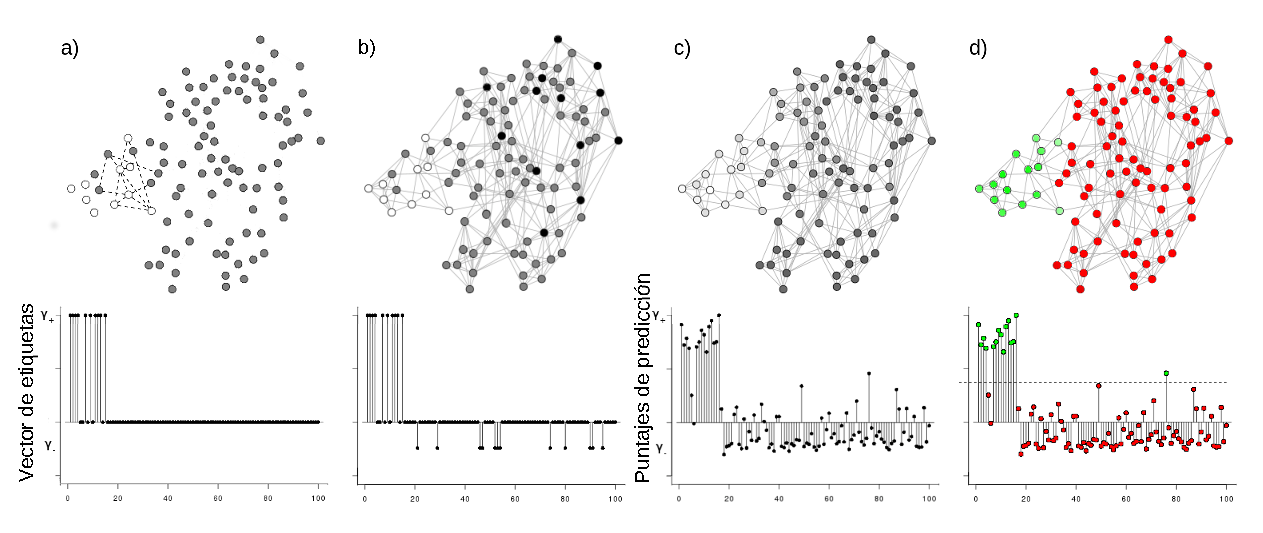
\includegraphics[width=\linewidth]{fig/workflow.eps}
	\caption[Evolución del grafo]{evolución del grafo, el vector de etiquetas y el vector de puntajes de predicción en los 4 pasos del método propuesto: a) Construcción de grafo; b)
	inicialización de conjunto negativo; c) Estimación de puntajes de predicción; d) optimización del umbral.}
	\label{fig:workflow}
\end{figure}
%****************************************************************************************

MiRNAss recibe como entrada un conjunto de vectores de características $m$-dimensional $\mathbf{x}_{i}$, que representan secuencias, y un vector
correspondiente de etiquetas $\Bell$. El elemento $i$-th en el vector de etiquetas tiene un valor positivo $\gamma_{+}$ si la secuencia $i$-th es un pre-miARN
conocido, un valor negativo $\gamma_{-}$ si no es un pre-miARN, y cero si es una secuencia desconocida que debe ser clasificada por el método. El método
tiene cuatro pasos: 1) construcción de un grafo donde cada nodo representa una secuencia; 2) buscar ejemplos negativos, si no se proporcionan; 3) estimación
de los puntajes de predicción para cada nodo en el grafo; y 4) estimación de un umbral óptimo para finalmente separar las secuencias en dos clases. Cada
paso se explica en detalle en las siguientes subsecciones.

La Figura~\ref{fig:workflow} muestra un ejemplo de la evolución del método. En este ejemplo, 15 secuencias son verdaderos pre-miARN y el resto son secuencias
no pre-miARN. En la Figura.~\ref{fig:workflow}.a, el grafo se construye y se asignan los valores iniciales a $\Bell$: valores positivos ($\gamma_{+}$) a los
ejemplos conocidos de pre-miARNs. En la Figura.~\ref{fig:workflow} .b, algunos nodos que están topológicamente lejos de los ejemplos positivos se etiquetan como
ejemplos negativos ($\gamma_{-}$). Los nodos del grafo están coloreados de acuerdo con los valores en el vector $\Bell$. En la Figura.~\ref{fig:workflow}.c,
los puntajes de predicción se estiman para todas las secuencias, teniendo en cuenta que: i) tienen que ser suaves; es decir, las secuencias topológicamente
cercanas en el gráfico deben tener puntajes de predicción similares; y ii) los puntajes tienen que ser similares a los valores distintos de cero dados en el
vector de etiqueta $\Bell$. Finalmente, usando los puntajes de predicción asignados a los ejemplos marcados, se estima un umbral óptimo para separar los
pre-miARN de las otras secuencias. Las secuencias que pasan el umbral están coloreadas en verde; el resto, en rojo.

\subsection{Construcción del grafo}

Para construir el grafo, donde cada nodo representa una secuencia y cada arista une dos nodos si las secuencias son similares en el espacio de las
características. Para medir la similaridad se utiliza la distancia euclidiana entre los vectores de características. Si una característica no ayuda
realmente a discriminar entre clases, puede empeorar el rendimiento del clasificador. Por lo tanto, es importante preprocesar los vectores de características
para ponderar adecuadamente cada característica de acuerdo con su poder de predicción. Un algoritmo que ha demostrado mejorar los resultados en
clasificadores que son sensibles a la función de distancia es el algoritmo RELIEF-F \citep{kononenko1994estimating, wettschereck1997review}. Además, es
computacionalmente eficiente y puede usarse para grandes volúmenes de datos.

Funciona de la siguiente manera: comenzando con un vector de pesos con $m$ ceros, para cada ejemplo busca el ejemplo más cercano de la misma clase y el
ejemplo más cercano que pertenezca a la otra clase. Luego, aumenta los pesos de las características que son similares al ejemplo de la misma clase y
diferente al ejemplo de la otra clase. Por el contrario, se reducen los pesos de las características que son diferentes al ejemplo de la misma clase o similar
al ejemplo de la otra clase. El resultado se llama vector de relevancia y tiene valores altos para las características más discriminativas. Si la relevancia
de una característica es negativa, no ayuda a discriminar entre clases; por lo tanto puede ser eliminada. El resto de las características se escala por su
puntaje de relevancia para dar más peso a las más discriminativas.

Para la construcción del grafo, una opción común es el algoritmo de $k$-vecinos más cercanos (KNN), dado que es simple, rápido, eficiente en uso de
memoria y fácilmente paralelizable. KNN construye una matriz de adyacencia ponderada por similitud con elementos

\begin{equation}
	a_{ij} =
	\begin{cases}
		\frac{\mu}{\mu + ||\mathbf{x}_{i} - \mathbf{x}_{j}||^2} & \text{si} \ \mathbf{x}_{j} \in  \mathcal{K}(\mathbf{x}_{i}) \ \text{y} \ \ell_{i}
		\ell_{j} \geq 0 \\
		0 & \text{en otro caso,} \\
	\end{cases}
\end{equation}

\noindent donde $\mathbf{x}_{i}$ es el vector de características correspondiente a la secuencia $i$-th, $\mathcal{K} (\mathbf{x}_{i})$ es el conjunto de los
$k$ vecinos más cercanos de $\mathbf{x}_{i}$, y $\mu$ es la media de las distancias entre las secuencias conectadas y se  utiliza para normalizar los pesos de
las aristas.

\subsection{Búsqueda de ejemplos negativos}

\renewcommand{\algorithmicrequire}{\textbf{Entrada:}}
\renewcommand{\algorithmicensure}{\textbf{Salida:}}
\renewcommand{\algorithmicrepeat}{\textbf{repetir}}
\renewcommand{\algorithmicuntil}{\textbf{mientras}}
\renewcommand{\algorithmicreturn}{\textbf{delvolver}}
\begin{algorithm}[tpb]
	\caption{Búsqueda automática de ejemplos negativos}
	\label{algNS}
	\begin{algorithmic}[1]
		\REQUIRE{matriz de adyacencia $A$, vector de etiquetas $\Bell$ con ceros y valores positivos únicamente, número de ejemplos negativos a etiquetar $T$.}
		\ENSURE{el vector $\Bell$ con $T$ etiquetas negativas asignadas.}
		\STATE{$s_{i} = \begin{cases}
				1 & \text{si} \quad \ell_{i} > 0 \\
				0 & \text{en otro caso} \\
		\end{cases}$}
		\REPEAT
		\STATE{$s_{i} = \max_{\forall j \neq i}\limits \, \{s_{i}, a_{ij} s_{j} \}, \quad \forall i$}
		\UNTIL{no hay cambios en $\mathbf{s}$}
		\STATE{$p_i=e^{1-s_i}-1,\quad \forall i$}
		\STATE{Muestrear $T$ elementos de $\Bell$ usando $\mathbf{p}$ como pesos para la selección}
		\STATE{Etiquetar elementos elegidos como clase negativa}
		\RETURN $\Bell$
	\end{algorithmic}
\end{algorithm}

Si solo se cuenta con ejemplos positivos, la matriz de adyacencia se puede utilizar para etiquetar un conjunto de secuencias como ejemplos negativos. La idea
clave es seleccionar aleatoriamente algunas secuencias sin etiqueta entre las más disímiles de los ejemplos positivos. De esta forma, la probabilidad de
etiquetar incorrectamente un pre-miARN bien conocido como un ejemplo negativo será baja. Para ello, se calcula una medida de la similitud de cada secuencia
con los ejemplos positivos utilizando la distancia topológica. Este vector de similitud, llamado $\mathbf{s}$, se inicializa con $+1$ en los elementos
correspondientes a ejemplos positivos. Los nodos sin etiqueta se inicializan con $0$. Entonces, se puede usar un método iterativo para actualizar las
similitudes en $\mathbf{s}$ (ver Algoritmo~\ref{algNS}). En cada iteración y para cada nodo, el valor de similitud correspondiente de cada vecino se
multiplica por los pesos de aristas correspondientes que los conectan. El valor máximo de los resultados obtenidos para cada vecino se compara luego con el
valor de similitud actual del nodo. Si es más alto, se actualiza el valor de similitud del nodo. Cuando no hay más cambios en $\mathbf{s}$, se seleccionan
$T$ secuencias de forma aleatoria usando como probabilidad de selección $p_{i} = e^{1 - s_{i}} -1$ y se etiquetan como ejemplos negativos.

\subsection{Estimación de puntajes de predicción}

En el tercer paso, los puntajes de predicción se calculan resolviendo un problema de optimización \citep{joachims2003transductive}. Como se dijo
anteriormente, se deben considerar dos puntos: i) los puntajes de predicción deben ser topológicamente suaves; y ii) las predicciones deben ser similares a
las etiquetas conocidas. Para suavizar la predicción, se minimiza el cuadrado de las diferencias entre las puntuaciones de predicción de las secuencias
adyacentes. Una representación conveniente para calcular fácilmente estas diferencias es el laplaciano normalizado del grafo \citep{shi2000normalized}, definido
como

\begin{equation*}
	L=I-D^{-1/2}AD^{-1/2}
\end{equation*}

\noindent donde

\begin{equation*}
	D_{ij} =
	\begin{cases}
		\sum_{k=0}^n A_{ik} & \text{si } i=j \\
		0 & \text{en otro caso} \\
	\end{cases}
\end{equation*}

El Laplaciano tiene una propiedad útil para medir la suavidad de la solución. Supongamos $\mathbf{z} \in \mathbb{R} ^ N$, con una predicción para cada nodo
del gráfico. Entonces,

\begin{equation}
	\begin{split}
		\mathbf{z}^T L \mathbf{z} & = \mathbf{z}^T I \mathbf{z} - \mathbf{z}^T {D^{-1/2}}^T A D^{-1/2} \mathbf{z} = \\
					  & = \sum_{i}^{n} z_{i}^{2} -  \sum_{i}^{n}  \sum_{j}^{n} \frac{z_{i}}{\sqrt{d_{ii}}} \frac{z_{j}}{\sqrt{d_{jj}}}
		a_{ij} = \\
		& = \frac{1}{2} \sum_{i}^{n} \sum_{j}^{n} a_{ij} \left(\frac{z_{i}}{ \sqrt{d_{ii}}} - \frac{z_{j}}{\sqrt{d_{jj}}}
	\right)^{2}.
\end{split}
\end{equation}

\noindent Esta última expresión muestra que $\mathbf {z} ^ T L \mathbf {z}$ mide la diferencia al cuadrado entre las predicciones $z_{i}$ y $z_{j}$,
ponderados por $a_{ij} $. Si las secuencias $ i $ y $ j $ son similares, y por lo tanto $ a_{ij} $ tiene un valor relativamente alto, cualquier diferencia
entre las dos predicciones tendrá un alto costo. Si no hay arista que conecte las dos secuencias, $a_{ij} = 0 $ y la diferencia entre las predicciones se
ignora. Además, se debe tener en cuenta que las predicciones se ponderan por el inverso de la raíz cuadrada del grado del nodo. Como resultado, los nodos con
un grado pequeño se consideran tan importantes como los nodos altamente conectados.

Para minimizar la inconsistencia entre las predicciones y las etiquetas conocidas, también se requiere la diferencia cuadrada entre las predicciones y las
etiquetas distintas de cero en $\Bell $. Por lo tanto, la función objetivo tiene dos términos: el primer término mide la falta de suavidad de la solución
usando la matriz laplaciana normalizada (componente no supervisada del aprendizaje), y el segundo término es la diferencia al cuadrado entre predicciones y
etiquetas distintas de cero en $\Bell$ (componente supervisada). Para aprovechar al máximo el aprendizaje semi-supervisado, no debe haber una gran
superposición entre las clases que se separarán. Sin embargo, si este requisito previo no se cumple, el primer término de la función objetivo no tendrá
ningún mínimo importante. Por lo tanto, el segundo término de la ecuación (el supervisado) conducirá la búsqueda. Por lo cual, si no hay una separación
clara entre las clases, el método se comportará de forma similar a cualquier otro método supervisado en las mismas condiciones.

El problema de optimización completo se define como

\begin{equation}
	\begin{split}
		\arg\min_{\mathbf{z}} & \qquad \mathbf{z}^TL\mathbf{z} +c(\mathbf{z}-\Bell)^TC(\mathbf{z}-\Bell) \\
		s.t. & \qquad \mathbf{z}^T\mathbf{1} = 0, \mathbf{z}^T\mathbf{z} = n,
	\end{split}
\end{equation}

\noindent donde la combinación de ambas restricciones evita soluciones triviales. En la primera restricción, se requiere que la suma de los elementos de
$\mathbf{z}$ sea cero; es decir, las etiquetas de predicción deben tener tanto valores negativos como positivos. La segunda restricción elimina las versiones
escaladas de la solución que, para nuestro propósito, son todas equivalentes.

Los valores $\ell_{i}$ se establecen en $\gamma_{+}$, $\gamma_{-}$ o cero, dependiendo de si la secuencia $ i $-th es positiva, negativa o desconocida,
respectivamente. Como la función objetivo obliga a los valores de $\mathbf{z}$ a acercarse a $\gamma_{+}$ o $\gamma_{-}$, estas constantes deben definirse de
manera tal que la solución óptima $\mathbf{z}^\star$ pueda satisfacer ambas restricciones del problema. Si $n_{+}$ y $n_{-}$ son los números verdaderos de
nodos positivos y negativos en la solución, definiendo $\gamma_{+} = \sqrt{n_{-}/n_{+}}$ y $\gamma_{-}=-\sqrt{n_{+}/n_{-}}$ hace $\mathbf{z}^\star$ satisfacer
ambas restricciones. Esto se puede observar al reemplazar $\mathbf{z}^\star$ en las restricciones y asumiendo que este vector tiene $n_{+}$ elementos iguales a
$\gamma_{+}$ y $n_{-}$ iguales a $\gamma_{-}$. Los números $n_{+}$ y $n_{-}$ son generalmente desconocidos, pero se pueden estimar fácilmente a partir de los
ejemplos disponibles. Si se proporcionan ejemplos positivos y negativos para el entrenamiento, se calculará $n_{+}/n_{-}$ como la proporción de ejemplos
dados. Si solo hay ejemplos positivos, $n_{+}$ se estima como el doble del número de secuencias de entrenamiento y $n_{-} = n - n_{+}$. Esta estimación
podría mejorarse utilizando el conocimiento del dominio, es decir, utilizando el número esperado de miARNs para una especie determinada; sin embargo, no es
necesario ya que el método propuesto no es sensible a estos parámetros (ver Figura~S1 en el Material Suplementario del Anexo~\ref{sec:mirnass}). Por lo tanto,
cualquier valor entre el número de secuencias de entrenamiento positivas y cuatro veces este número se puede utilizar sin impacto en el rendimiento. Por defecto,
se usa el doble del número de secuencias de entrenamiento positivas como valor intermedio.

La constante $ c $ en la función objetivo se puede usar para establecer el peso relativo del segundo término en comparación con el primero. Un valor grande
de $ c $ otorga una mayor penalización a las clasificaciones erróneas, lo que lleva los puntajes de predicción a valores similares a las etiquetas distintas
de cero $ \Bell $. Por el contrario, si se usa un valor bajo de $ c $, las clasificaciones erróneas son menos penalizadas y el primer término domina la
función objetivo, lo que produce una solución más suave. La matriz $C$ en el segundo término es una matriz diagonal que tiene valor cero en los elementos
correspondientes a secuencias desconocidas. De esta manera, las secuencias sin etiqueta se ignoran en este término. En los elementos distintos de cero
(correspondientes a los ejemplos etiquetados), el valor asignado permite diferentes penalizaciones por clasificación errónea para cada secuencia. Esta
ponderación puede usarse, por ejemplo, para asignar valores inferiores a los pre-miARN que no han sido validados experimentalmente o que son ejemplos
negativos poco confiables. También se puede usar para evitar la clasificación errónea de ejemplos etiquetados. En la Sección S2 del Material Complementario
del Anexo~\ref{sec:mirnass} se demuestra que si $ C_ {ii}> (n n _ {+}) / (c n _ {-}) $, la clasificación incorrecta de la secuencia $ i $ -th tendrá una mayor penalización
que cualquier penalización en el término no supervisado. Entonces, no puede ser mal clasificado. Como valor predeterminado, los elementos distintos de cero
de $ C $ se establecen en $ 1 $, tanto para los ejemplos positivos como negativos.

Para resolver este problema de optimización, primero calculamos la descomposición espectral del Laplaciano $ L = U \Sigma U ^ T $. A continuación,
utilizamos un nuevo vector de parámetro $ \mathbf {w} $ tal que $ \mathbf {z} = U \mathbf {w} $. Como el vector propio correspondiente al valor propio más
bajo siempre es constante, la primera restricción del problema de optimización se convierte en $ w_ {1} = 0 $. Si definimos $ V $ como la matriz con todos
los vectores propios, excepto el primero, y $ H $ como la matriz diagonal con todos los valores propios, excepto el más bajo, obtenemos el siguiente problema
de optimización

\begin{equation}
	\begin{split}
		\arg\min_{\mathbf{w}} & \quad \mathbf{w}^T H \mathbf{w} + c (V \mathbf{w} - \Bell)^T C (V \mathbf{w} - \Bell) \\
		s.t. & \quad \mathbf{w}^T \mathbf{w} = n.
	\end{split}
\end{equation}

\noindent Definiendo $ Q = H + c V ^ T C V $ y $ b = c V ^ T C \Bell $, este problema puede reescribirse como

\begin{equation}
	\begin{split}
		\arg\min_{\mathbf{w}} &\quad \mathbf{w}^T Q \mathbf{w} + 2 b^T \mathbf{w} + c \Bell^T C \Bell \\
		s.t. &\quad \mathbf{w}^T \mathbf{w} = n,
	\end{split}
\end{equation}

\noindent donde el último término se puede descartar dado que es constante. Usando los multiplicadores de Lagrange, el mínimo global de esta función se
produce en $\mathbf {w}^\star = (Q - \lambda^\star I)^{- 1} \mathbf{b} $. Ahora, usando los resultados de \cite{gander1989contrained}, $ \lambda^\star$
se puede calcular como el menor autovalor de

\begin{equation}
	M = \left( \begin{array}{cc}
			Q & -I \\
	\frac{{\mathbf{b} \mathbf{b}^T}}{{n}} & Q \end{array} \right).
\end{equation}

\noindent A partir de esta solución, las etiquetas se calculan como $ \mathbf {z} ^ \star = V \mathbf {w} ^ \star $.

\subsection{Umbralización de los puntajes de predicción}

Dados los altos desbalances que están presentes en los datos de un genoma completo, es necesario aumentar el costo de clasificación errónea de la clase
positiva. Mientras que la matriz $C$ se puede usar para asignar diferentes costos de clasificación errónea en el proceso de optimización, estimar el umbral
que se aplicará en $\mathbf{z}$ es un método más flexible ya que permite elegir la medida de rendimiento a maximizar. Dado que se espera que los puntajes de
predicción ordenen las secuencias de acuerdo a la probabilidad de ser pre-miARNs, modificar el umbral utilizado para separar las dos clases equivale a
clasificar con distintas ponderaciones por clase \citep{mease2007boosted}.

Una métrica de evaluación común que se usa en problemas con desbalance de clases es la media geométrica ($ \bar {G} $) de la sensibilidad y la
especificidad $ \bar {G} = \sqrt {S ^ {+} S ^ {-} } $ \citep{batuwita2009micropred, gudys2013huntmi}, donde $ S ^ {+} $ es la proporción de secuencias
positivas correctamente clasificadas como positivas (sensibilidad), y $ S ^ {-} $ es la proporción de secuencias negativas correctamente clasificadas como
negativas (especificidad). Esta medida tiene la ventaja de dar la misma importancia a las clases negativas y positivas, independientemente de la cantidad de
elementos en cada clase. Una mejor medida es el \mbox{F-score} $ F_ {1} = 2 \, P \, S ^ {+} / (P + S ^ {+}) $, donde $ P $ es la precisión, que es la
proporción de verdaderos positivos dentro de las secuencias clasificadas como positivas. Cuando se utiliza $ F_ {1} $ para la optimización del umbral, se
obtiene una mejor $ P $ a costa de una $ S ^ {+} $ más baja. Debido al gran desbalance de clases en este problema de clasificación, es importante prestar
especial atención a la cantidad de falsos positivos. Por lo tanto, $F_{1}$ es una mejor medida para este problema.

Los puntajes de predicción obtenidos para los ejemplos etiquetados se pueden usar para encontrar el umbral que maximice cierta medida de rendimiento objetivo.
Debe señalarse que esto es solo una estimación, ya que se desconoce la clase a la que pertenecen real las secuencias no etiquetadas. Por esta razón, si
ordenamos los puntajes de predicción $ \mathbf {z} ^ \star $ y calculamos la medida de desempeño utilizando como umbral cada valor de este vector,  entre dos
ejemplos etiquetados consecutivos aparecerán regiones donde esta medida se hace constante. Si el número de ejemplos etiquetados es bajo, estas regiones
constantes pueden ser relativamente grandes. Por lo tanto, el umbral final se establece como el punto medio entre el puntaje de predicción más alto y más
bajo  donde se maximice la medida de rendimiento (ver Figura~\ref{sec:mirnass}). Una vez que se realiza una predicción, se pueden agregar nuevos
nodos al grafo etiquetado usando algoritmos rápidos para encontrar los k-vecinos más cercanos \citep{malkov2014approximate}. Esto permite realizar
predicciones sobre nuevas secuencias o extraer información de datos sin procesar mediante el análisis de sus adyacencias \citep{chapelle2006semi}.


\chapter{Resultados} \label{sec:results}

\section{Procesamiento de secuencias de ARN de tipo tallo-horquilla}

Se ha desarrollado una herramienta llamada HextractoR, simple e integrada, que automáticamente extrae y pliega todas las secuencias de horquilla a partir de
datos brutos del genoma completo. El método propuesto aprovecha los últimos avances en la predicción de estructuras secundarias. Al procesar grandes
ventanas superpuestas, no se pierden ni se cortan de manera inapropiada las horquillas. Permite procesar genomas en paralelo y con pocos requisitos de memoria,
ya que puede dividir automáticamente archivos fasta demasiado grandes.

Se procesaron varios genomas y los resultados se compararon con los del programa mirCheck de EMBOSS \citep{olson2002emboss}. La Tabla~\ref{tab:hextractor} muestra los
resultados del procesamiento de 6 genomas completos: \textit{Homo sapiens}, \textit{Arabidopsis thaliana}, \textit{Danio rerio}, \textit{Anopheles gambiae} y
\textit{Caenorhabditis elegans}, además de otra especie menos estudiada: \textit{Echinococcus multilocularis}. Para cada uno, se muestra el número de
secuencias extraídas con mirCheck y HextractoR, en la segunda y tercera columna, respectivamente. Con respecto a los pre-miARNs en particular se informa, en
cada genoma analizado, en la cuarta columna de la tabla el número de pre-miARNs conocidos (de acuerdo con miRBase 21) para las 6 especies. La proporción de
aquellos encontrados por los métodos comparativos se muestra en las dos últimas columnas. Se puede ver claramente que en todos los casos, el rendimiento de
HextractoR es superior. Además, en muchos casos, el 100 \% de los pre-miARNs conocidos se extraen correctamente.

Las diferencias en cantidad de pre-miARNs encontrados que muestra la Tabla~\ref{tab:hextractor} se pueden deber a varios motivos. En primer lugar, como se ve en
la segunda y tercer columna, HextractoR consigue capturar más horquillas que mirCheck. Al utilizar ventanas solapadas de un tamaño varias veces mayor al de
una horquilla para recorrer el genoma, HextractoR consigue capturar cualquier horquilla. MirCheck se podría configurar para que utilice ventanas con una mayor
longitud, pero en ese caso descartaría la mayoría de las secuencias porque estas formarían estructuras con varios bucles y mirCheck no realiza el proceso de
separación en horquillas como si lo hace HextractoR.

\begin{table}[t]
	\centering
	\small
	\begin{tabular}{l r r r r r c}
		\toprule
		\multirow{2}{*}{Especies} & \multicolumn{2}{c}{Horquillas extraídas}  & & \multicolumn{2}{c}{pre-miARNs encontrados}    &    pre-miARNs  \\ \cmidrule{2-3} \cmidrule{5-6}
						    &    Einverted  &       HExtractor     & & Einverted     &   HExtractor  &  conocidos \\ \cmidrule{1-7}
		\textit{Anopheles gambiae}          &  1.410.532    &  \textbf{4.276.543}  & &  92,42 \%     &    \textbf{100,00  \%}       &   66        \\
		\textit{Caenorhabditis elegans}     &    875.588    &  \textbf{1.739.124}  & &  90,00 \%     &     \textbf{99,60  \%}       &  250        \\
		\textit{Danio rerio}                & 11.028.128    & \textbf{23.214.338}  & &  93,06 \%     &     \textbf{99,42  \%}       &  346        \\
		\textit{Echinococcus multilocularis}&    509.530    &  \textbf{1.898.911}  & &  81,81 \%     &    \textbf{100,00  \%}       &   22        \\
		\textit{Arabidopsis thaliana}       &    874.320    &  \textbf{1.357.455}  & &  91,69 \%     &     \textbf{94,77  \%}       &  325        \\
		\textit{Homo sapiens}               & 18.654.426    & \textbf{48.206.494}  & &  85,38 \%     &     \textbf{97,45  \%}       & 1881        \\
		\bottomrule
	\end{tabular}
	\label{tab:hextractor}
	\caption[Cantidad de horquillas y pre-miARN en varios genomas]{cantidad de horquillas y pre-miARNs encontrados por cada método en el genoma de 6 especies}
\end{table}

\section{Predicción de pre-microARN}

En esta sección se presentan los resultados de los experimentos realizados para probar el rendimiento de miRNAss en diferentes condiciones. En la primera
subsección, se reprodujeron experimentos realizados por otros autores para comparar miRNAss con métodos supervisados del estado del arte en condiciones
controladas. Los conjuntos negativos fueron definidos artificialmente por los autores originales y la proporción de ejemplos etiquetados fue muy alta. En la
segunda subsección, el porcentaje de ejemplos etiquetados se redujo gradualmente para acercarse más a un caso real de predicción de pre-miARN. Además,
miRNAss se probó en un esquema de una clase, donde solo se conocían ejemplos positivos (pre-miARNs reales) de antemano. En la última subsección, miARN se
aplicó a una tarea de predicción real a partir de datos del genoma completo de 3 especies modelo, sin ejemplos negativos y utilizando solo un bajo número de
ejemplos positivos. En esta última prueba, había un enorme desbalance de clases y se procesaron más de un millón de secuencias de entrada.
Comparación en conjuntos de datos etiquetados artificialmente

\subsection*{Comparación con métodos del estado del arte}
Las condiciones experimentales en esta sección son las mismas que las utilizadas para probar otros métodos del estado del arte. Se estableció $ F_{1} $ como
medida de desempeño utilizada para la optimización del umbral en todos los métodos. Los experimentos se diseñaron para estimar el desempeño de métodos de
aprendizaje supervisado, por lo que se utiliza un esquema estándar de validación cruzada con 10 particiones. En este esquema, la mayoría de las secuencias
están etiquetadas artificialmente para el entrenamiento, y solo un $ 10 \% $ queda sin etiquetar. Por lo tanto, es importante señalar que la principal
ventaja del aprendizaje semi-supervisado, que es explotar datos no etiquetados para mejorar los resultados, no se puede aprovechar en estos experimentos.
Para una comparación justa, en estos experimentos los clasificadores usan las mismas características. Este conjunto está compuesto por 7 características de
miPred \citep{ng2007novo}, más 14 de microPred \citep{batuwita2009micropred} y 7 añadidas por \cite{gudys2013huntmi}. Para obtener más detalles sobre el
conjunto de características, consulte la Sección S4 del Anexo~\ref{sec:mirnass}.

Como antes se especificó, se ejecutó una validación cruzada estratificada de 10 particiones en cinco conjuntos de datos y se compararon los resultados con
los obtenidos por HuntMi \citep{gudys2013huntmi}. Las particiones fueron construidas al azar usando una semilla fija para tener experimentos totalmente
reproducibles. Tres conjuntos de datos contenían una mezcla de secuencias de diferentes especies, que se agruparon en los conjuntos de datos animales (10
especies), plantas (7 especies) y virus (29 especies). Los otros dos conjuntos de datos contenían secuencias de \textit{Homo sapiens} y \textit{Arabidopsis
thaliana}. Los parámetros utilizados en miRNAss fueron los mismos en todas las pruebas: $ c = 1 $ y $ k = 10 $ (tanto para RELIEF-F como para la construcción
de grafos). MiRNAss se probó con y sin RELIEF-F, para medir su impacto en el rendimiento. La ponderación de características obviamente se calculó
utilizando solo los datos de entrenamiento de cada partición.


Los tiempos transcurridos medidos \footnote{Intel \textregistered Core \texttrademark i5-4460 CPU @ 3.20GHz, 8 GB de RAM.} En cada pliegue se promediaron y se
presentan en la Tabla~\ref{tab:times}. La primera columna muestra el número total de secuencias. La segunda y tercera columnas indican el número de
secuencias pre-miARN y no pre-miARN en cada conjunto de datos. La cuarta y quinta columnas presentan los tiempos transcurridos para cada método. La última
columna muestra el cociente entre el tiempo que tardó HuntMi y el tiempo que tardó miRNAss. La mayor diferencia se observó en el conjunto de datos más
pequeño (virus): miRNAss fue 38 veces más rápido que HuntMi. Arabidopsis es el segundo conjunto de datos más pequeño, y aquí miRNAss fue 14 veces más
rápido. En los siguientes tres conjuntos de datos, las diferencias de tiempo de computación entre miRNAss y HuntMi aumentaron a medida que crecía el número
de secuencias. Estos resultados muestran que miARN no solo es mucho más rápido sino que el costo computacional crece más rápido en HuntMi. Tales
diferencias pueden ser irrelevantes en pequeños conjuntos de datos como los que se utilizan en esta subsección, pero se vuelven muy importantes en tareas de
predicción de genoma completo, donde se procesan varios millones de secuencias. Por ejemplo, si extrapolamos los tiempos de entrenamientos utilizando los
datos de la tabla, para entrenar a HuntMi con 1.7 millones de secuencias (uno de los conjuntos de datos del genoma utilizado en la sección~\ref{sec:results:genome-wide})
se necesitarían alrededor de 37 días, mientras que miRNAss solo se requieren 18 horas.
Con respecto a las medidas de predicción, ambos métodos se realizaron de manera similar en este experimento. Se aplicó una prueba de Friedman \citep{friedman1937use},
que dio como resultado un valor $ p $ de 0,179. Esto demuestra que el método propuesto puede obtener resultados equivalentes a un método
del estado del arte para la configuración supervisada, aunque en menos tiempo (como se muestra en la Tabla~\ref{tab:times}).
\begin{table}[t]
	\small
	\centering
	\begin{tabular}{@{}lrrrrrrr@{}} \toprule
		&  \multicolumn{3}{c}{Número de secuencias} & & \multicolumn{3}{c}{Tiempos} \\ \cmidrule{2-4} \cmidrule{6-8}
		Conjunto de datos     &   Total  &   miARN   &  no-miARN& &  HuntMi  & miRNAss & \textit{speedup} \\\midrule
		Virus       &   1,076  &      237  &       839 & &     38 s &     1 s & 38.00    \\
		Arabidopsis &  28,590  &      231  &    28,359 & &  1,819 s &   129 s & 14.10    \\
		Human       &  82,634  &    1,406  &    81,228 & &  9,873 s &   462 s & 21.37    \\
		Plants      & 117,101  &    2,172  &   114,929 & & 21,561 s &   714 s & 30.19    \\
		Animals     & 225,207  &    7,053  &   218,154 & & 65,762 s & 1,834 s & 35.85    \\\bottomrule
	\end{tabular}
	\caption[Comparación de tiempos de ejecución]{comparación de los tiempos de ejecución entre miRNAss y HuntMi.\label{tab:times}}
\end{table}
Además, fue posible verificar que RELIEF-F mejoró los resultados en todas las pruebas, aunque en algunas de ellas las diferencias fueron pequeñas. Esto era
de esperar, dado que las características utilizadas en estos conjuntos de datos son el resultado de procesos previos de selección de características. Una
prueba de Friedman en esta comparación da como resultado un valor $ p $ de 0.025, lo que demuestra que las diferencias son significativas. Se pueden ver más
detalles sobre estos resultados en la Figura~S5 del Anexo~\ref{sec:mirnass}.

Para probar la capacidad de miRNAss para predecir nuevos pre-miARNs en diferentes especies, los pre-miARNs conocidos de animales y plantas que se incluyeron en
la versión 17 de mirBase se usaron para el entrenamiento, y los pre-miARNs que se agregaron en versiones 18 a 19 fueron usados como conjunto de prueba. En el caso de las especies
animales, se añadió microPred \citep{batuwita2009micropred} en la comparación, ya que era el mejor software para la predicción de miARN humano en el
momento de su publicación. En plantas, el método agregado fue PlantMiRNAPred \citep{xuan2011plantmirnapred}, porque está específicamente diseñado para
especies de plantas. Cabe señalar que, una vez más, el porcentaje de secuencias no etiquetadas en el conjunto de datos es muy bajo: menos del 0,3 \% en
animales y menos del 1,3 \% en plantas.
\begin{figure}[t]
	\centering
	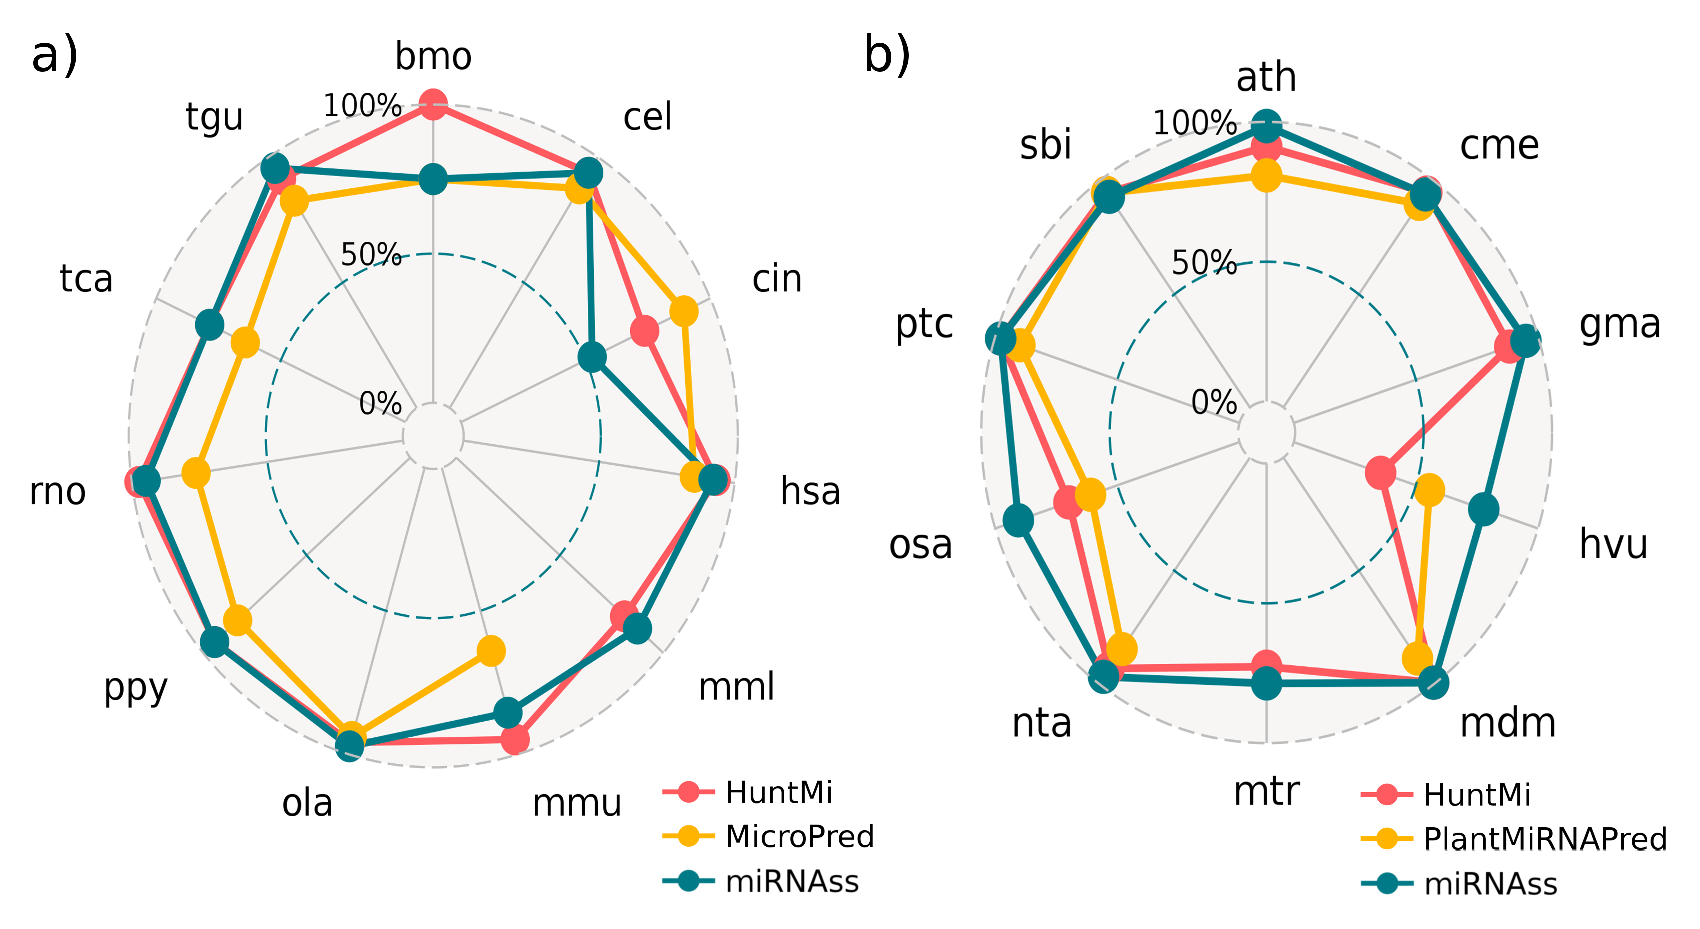
\includegraphics[width=0.6\linewidth]{fig/delta_mirbase_radar.eps}
	\caption[Sensibilidad en animales y plantas]{sensibilidad obtenida con varios clasificadores del estado del arte en: a) animales, y b) plantas.
		La distancia de cada punto al centro mide la sensibilidad obtenida obtenida cada especie.}
	\label{fig:deltaRadar}
\end{figure}
La $S^{+}$ obtenida para cada especie se muestran en la Figura~\ref{fig:deltaRadar}, donde cada clasificador se muestra con un color diferente a través de una
gráfica de radar. En el conjunto de datos de animales, miRNAss superó a microPred en casi todas las especies. En el conjunto de datos humanos, miRNAss obtuvo
una mayor $S^{+}$ que microPred, que, como se mencionó anteriormente, se diseñó específicamente para humanos. Comparado con HuntMi, miRNAss obtuvo mayores
$S^{+}$ en 4 especies, HuntMi produjo mejores resultados en 4 especies y los resultados obtenidos fueron iguales en 3 especies. En plantas, miRNAss superó a
PlantMiRNAPred en casi todas las especies. Comparado con HuntMi, miRNAss tuvo una mejor $S^{+}$ en 8 especies, mientras que HuntMi superó ligeramente al
miRNAss en solo 2 especies (\textit{Cucumis melo} y \textit{Sorghum bicolor}).
Para analizar si hubo diferencias significativas entre los clasificadores, se realizaron pruebas de Nemenyi \citep{nemenyi1962distribution} para ambos
conjuntos de datos ($ p<0,05 $). En las especies de animales, HuntMi y miRNAss produjeron resultados equivalentes, pero ambos se desempeñaron mejor que
microPred. En especies de plantas, miRNAss obtuvo el rango más bajo (el mejor) y una diferencia significativa con PlantMiRNAPred. Sin embargo, la diferencia
con HuntMi no fue estadísticamente significativa.

Los métodos supervisados hacen un uso extenso de los datos etiquetados, no solo para el entrenamiento sino también para encontrar los hiper-parámetros
y umbrales óptimos. Por el contrario, miRNAss se diseñó sobre la hipótesis de que los ejemplos etiquetados son escasos, poco confiables y no
representativos de toda la clase, que en realidad es un escenario más realista para esta tarea de predicción. Por lo tanto, debe tenerse en cuenta que,
incluso bajo estas condiciones desfavorables, miRNAss obtuvo resultados significativamente mejores que MicroPred y PlantMiRNAPred, y resultados equivalentes a
los producidos por HuntMi, siendo sin embargo, mucho más rápido.

\subsection*{Pocos ejemplos etiquetados}

\begin{figure}[t]
	\centering
	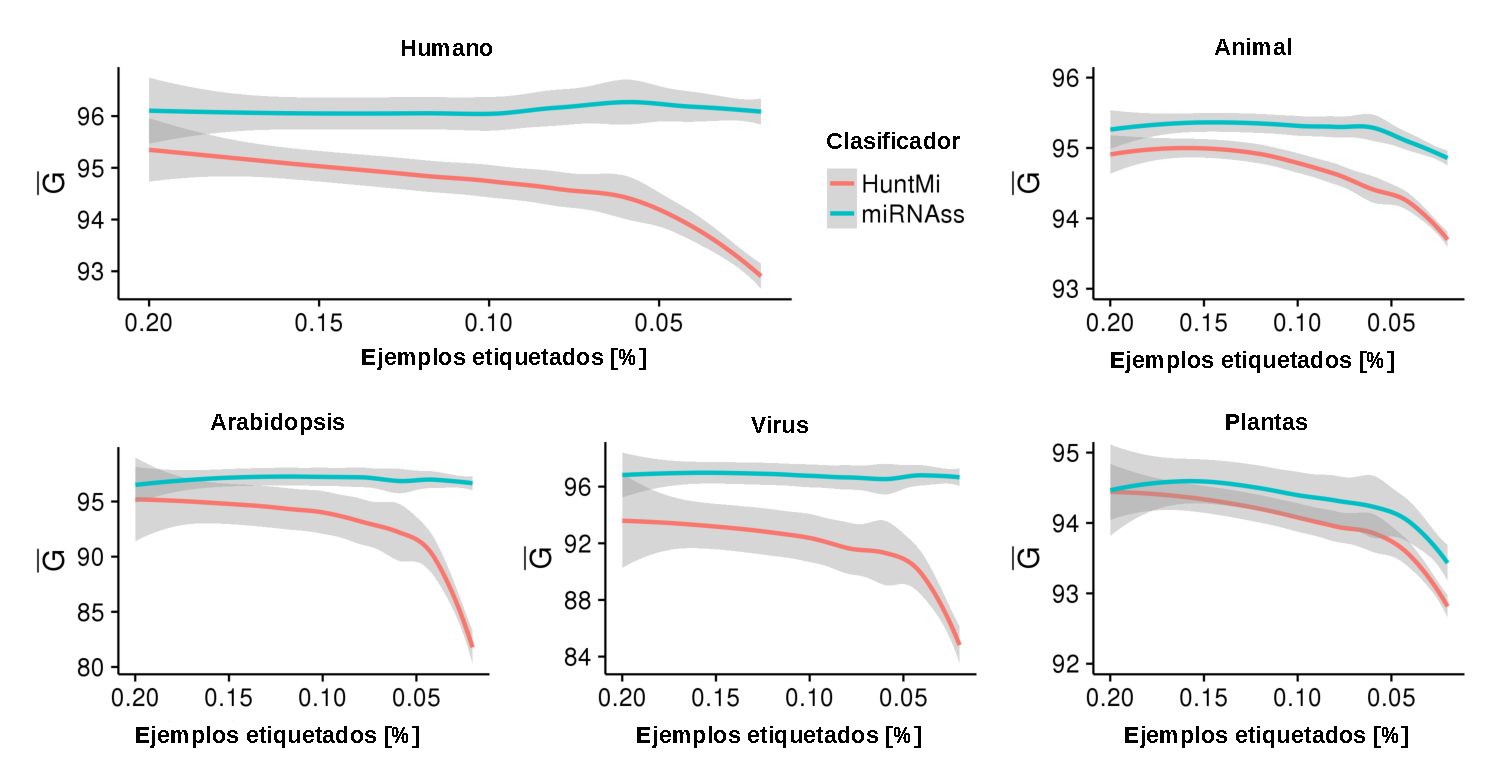
\includegraphics[width=\linewidth]{fig/few_labeled-huntmi.eps}
	\caption[$\bar{G}$ con pocos ejemplos de entrenamiento]{curvas de $\bar{G}$ obtenidas al disminuir el porcentaje de ejemplos etiquetados. Regiones
		sombreados representan los intervalos de confianza de la estimación con regresión local (LOESS) con $p < 0.05$.}
	\label{fig:fewSamples:huntmi}
\end{figure}

Para representar un escenario más realista en el que el número de ejemplos conocidos es bajo, los cinco conjuntos de datos utilizados en las últimas pruebas
se utilizaron con distintos porcentajes de secuencias etiquetadas y se realizaron pruebas en un esquema de validación entrenamiento-prueba. El porcentaje de
ejemplos etiquetados se redujo del 20 \% al 2 \%, con un paso del 2 \%. Los ejemplos etiquetados se seleccionaron al azar y las pruebas se repitieron 200 veces
para cada porcentaje para estimar los intervalos de confianza. En la Figura~\ref{fig:fewSamples:huntmi}, se estimaron las curvas de $F_{1}$ esperadas con
intervalos de confianza de 0,05 para la comparación. En el conjunto de datos humanos, el $F_{1}$ es casi un 10 \% más alto para miRNAss, independientemente
del porcentaje de secuencias marcadas. En el conjunto de datos de Arabidopsis, donde el número de secuencias de ejemplos positivos fue menor, las diferencias
a favor de miRNAss fueron más altas en los porcentajes más bajos de ejemplos etiquetados, lo que indica que miRNAss puede identificar efectivamente la clase
positiva incluso con un número muy bajo de ejemplos. Las mismas tendencias se observan en los animales, las plantas y los conjuntos de datos de virus.
Estos resultados no solo muestran que miRNAss es capaz de superar a los métodos supervisados cuando el número de ejemplos etiquetados es bajo, sino
también que las tasas de error estimadas usando una alta proporción de ejemplos etiquetados son muy diferentes de las obtenidas en escenarios más realistas.

Un paso más hacia una tarea de predicción más realista consiste en usar solo ejemplos positivos. Bajo estas condiciones, miRNAss se comparó con miRank
\citep{xu2008microrna}, que fue diseñado para trabajar con un número extremadamente pequeño de ejemplos positivos. Se utilizaron los conjuntos de datos
proporcionados por el autor original: 533 pre-miARNs humanos y 1000 secuencias no miARN. Para hacer una comparación justa, ambos métodos usaron el conjunto
de características de miRank. Este conjunto está compuesto por 32 tripletas \citep{xue2005classification}, MFE normalizado, propensiones de emparejamiento de
bases normalizadas de ambos brazos y longitud de bucle normalizado. Se marcó un número variable de ejemplos positivos (1, 2, 4, 8, 16, 32, 64 y 128) y el
resto de las secuencias se dejaron sin etiquetar para medir las tasas de error. Como los resultados dependen de un muestreo aleatorio de las secuencias, este
procedimiento se repitió 1000 veces para cada número de ejemplos etiquetados. MiRank proporciona como resultado una puntuación continua; por lo tanto, se
utilizaron los puntajes de predicción obtenidos con miRNAss en lugar de utilizar las clases. Se calculó el área bajo la curva de precisión-recuperación
(AUCPR, del ingles \textit{Area Under Precision-Recall Curve}), para realizar una comparación independiente del umbral utilizado para definir las clases
\citep{bradley1997use}.
La figura~\ref{fig:miRank} presenta un diagrama de caja con la distribución de AUCPR obtenida por cada clasificador para diferentes cantidades de ejemplos
etiquetados. MiRNAss mantuvo una AUCPR casi constante, independientemente del número de pre-miARNs marcados, mientras que el rendimiento de miRank disminuyó
marcadamente. Además, los valores de AUCPR para miRNAss mostraron pequeña dispersión en comparación con miRank, que se vuelve muy inestable cuando
disminuye el número de ejemplos etiquetados. Esta inestabilidad puede ser producida por ejemplos positivos que están cerca de la frontera de la clase, lo que
hace que miRank no establezca correctamente la frontera de decisión. El algoritmo semi-supervisado de miRNAss logró encontrar correctamente las regiones de
baja densidad que separan los miARNs del resto de las secuencias, independientemente de los ejemplos proporcionados.

\begin{figure}[tpb]
	\centering
	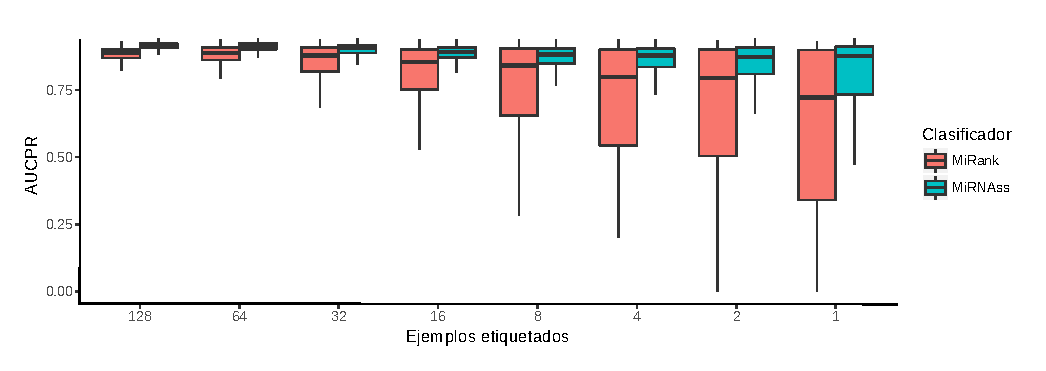
\includegraphics[width=\linewidth]{fig/few_samples_miRank.eps}
	\caption[$AUC$ con pocos ejemplos positivos]{diagrama de caja de las AUC obtenidas por miRNAss y miRank, con diferentes cantidades de ejemplos de entrenamiento positivos.}
	\label{fig:miRank}
\end{figure}

\subsection*{Predicción real en genomas completos} \label{sec:results:genome-wide}

MiRNAss se probó con los datos genómicos de tres genomas bien conocidos: \textit{Arabidopsis thaliana}, \textit{Caenorhabditis elegans} y \textit{Anopheles
gambiae}, para reproducir todas las condiciones de una tarea de predicción real. Los genomas completos se procesaron para extraer todos las secuencias con
estructura secundaria tipo tallo-horquilla existentes. Para este propósito se utilizó HExtractor, la herramienta desarrollada para tal fin. Este proceso
dejó un total de 1.356.616 secuencias de \textit{A. thaliana}; 1,698,859 secuencias de \textit{C. elegans}; y 4,276,188 secuencias de \textit{A. gambiae}.
Para detectar los pre-miARNs conocidos se utilizó la base de datos mirBase v21. Esto definió un total de 304, 249 y 66 horquillas como conjunto positivo para
\textit{A. thaliana}, \textit{C. elegans}, \textit{A. gambiae}, respectivamente.
Se extrajeron dos conjuntos de características de los tres genomas. El primero (FS1) es el mismo usado en la Sección ~\ref{sec:results}.1, para hacer una
comparación justa con uno de los métodos. El segundo conjunto de características (FS2) es un conjunto ampliado compuesto por casi todas las características
propuestas para la predicción pre-miARN en la literatura. FS2 se calculó con miRNAfe y cada vector de característica resultó en 79 elementos. Para obtener más
información sobre los conjuntos de características, consulte la Sección~S4 del Anexo~\ref{sec:mirnass}. Se utilizó un esquema de validación cruzada (CV) de 10
veces para medir el rendimiento de miARNs con curvas ROC promediadas.
Muchos algoritmos de predicción pre-miARN se probaron en estos conjuntos de datos para comparar su rendimiento con miRNAss. En total se han probado once
predictores, pero la mayoría han fallado con datos genómicos o sus servidores no funcionan. Los cinco predictores que se pudieron aplicar a genomas completos
fueron HuntMi, Mirident \citep{liu2012integrated}, HHMMiR \citep{kadri2009hhmmir}, MiRPara \citep{wu2011mirpara} y miR-BAG \citep{jha2012mirbag}. Los primeros
dos métodos producen clasificaciones duras (en vez de puntajes continuos) por lo que se representan como puntos en las figuras ROC. Por otro lado, dado que
MiRPara, miR-BAG, HHMMiR y miARN proporcionan puntajes continuos, se dibujaron curvas ROC completas. MiR-BAG no se ejecutó en \textit{A. thaliana} porque no
proporciona un modelo pre-entrenado para plantas. Los puntajes de salida obtenidos con este método sólo pueden tomar cuatro valores posibles, por lo que las
curvas ROC contienen regiones constantes. Estos resultados se presentan en la Figura~\ref{fig:ROC}.

En el genoma de \textit{A. thaliana}, se puede ver que las curvas ROC de miRNAss están por encima de las curvas de miRPara y HHMMiR para todos los valores
umbral. Cabe señalar que Mirident, a pesar de tener la mayor tasa de positivos verdaderos (sensibilidad), también tiene la mayor tasa de falsos positivos.
HuntMi es más equilibrado, con un alto reconocimiento de secuencias positivas y un número moderado de falsos positivos. Sin embargo, está debajo de miRNAss
con cualquiera de los dos conjuntos de características.
En el genoma de \textit{C. elegans}, se puede hacer un análisis similar para HuntMi y Mirident. En este conjunto de datos, miR-BAG genera una curva ROC
similar a la curva de MiRPara, ambas debajo del resto de las curvas. HHMMiR presenta un mejor rendimiento que estos métodos, pero una vez más es superado por
miRNAss.
\begin{figure*}[tpb]
	\centering
	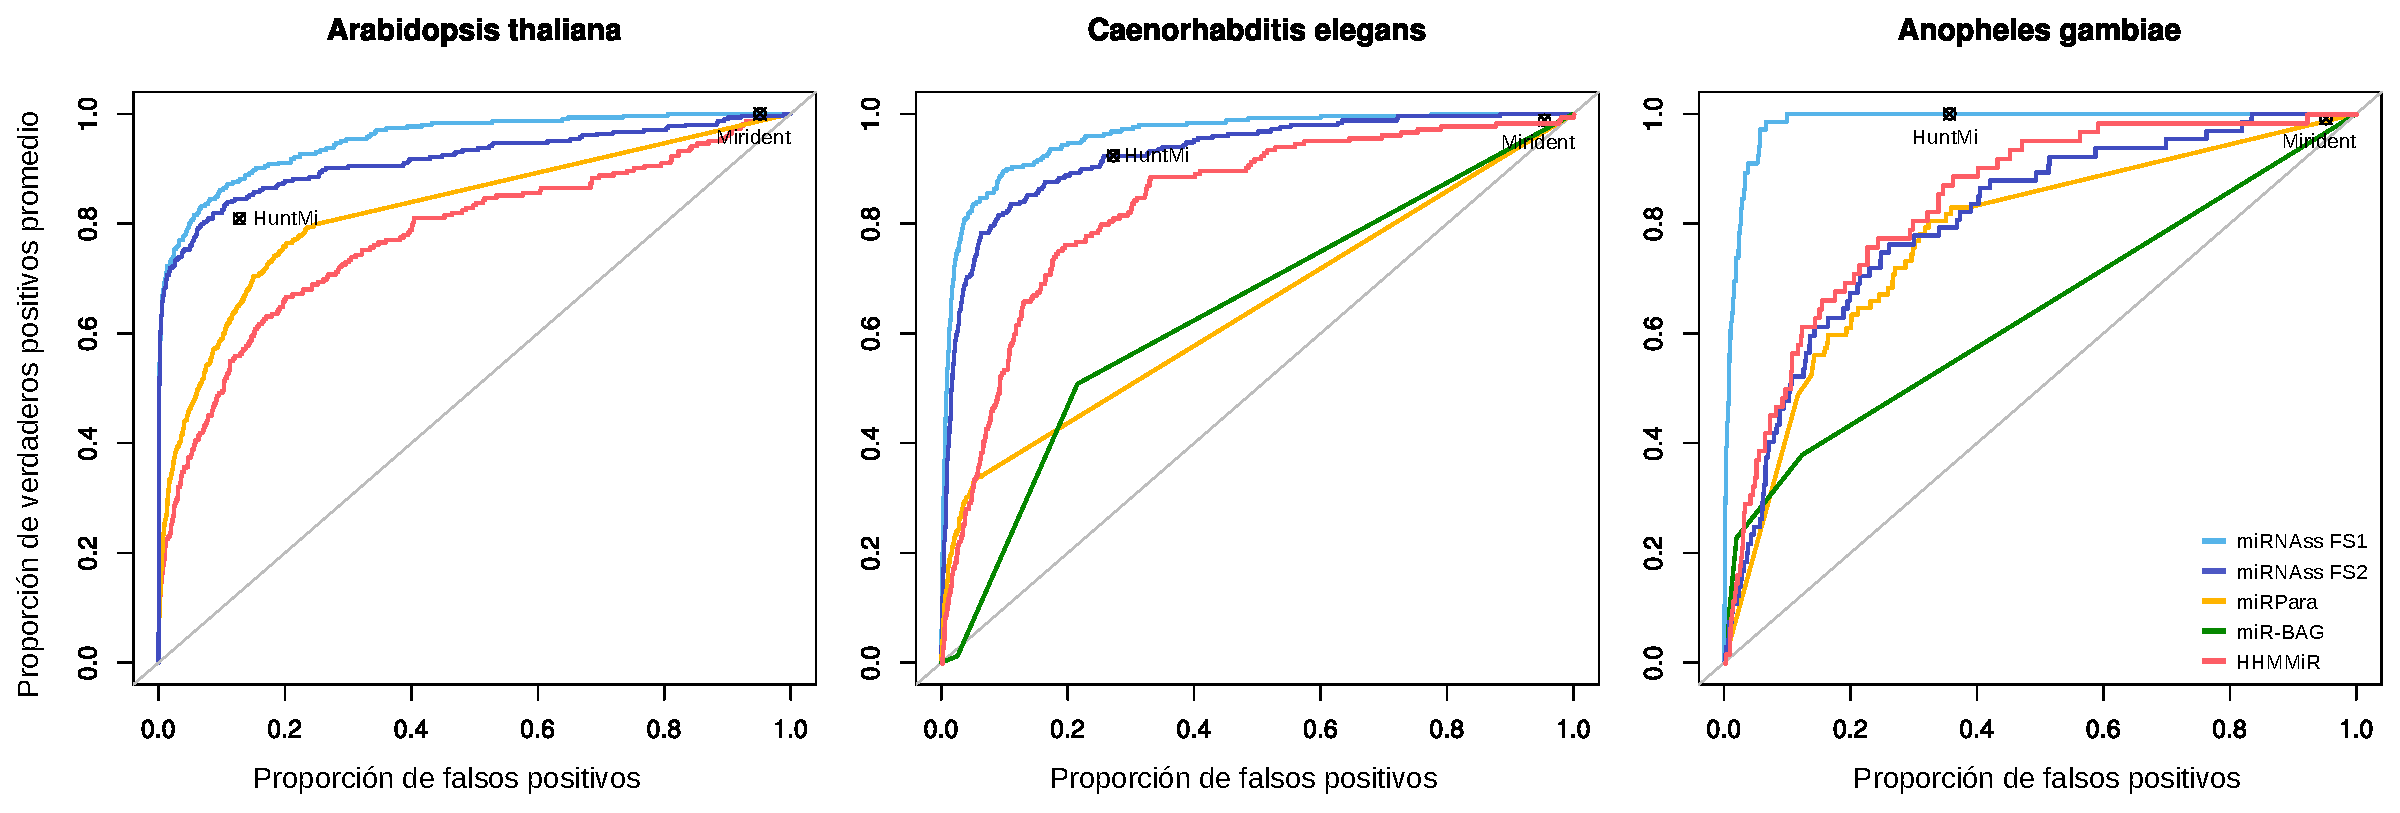
\includegraphics[width=\linewidth]{fig/genome-wide_ROC.eps}
	\caption[Curvas ROC en genoma completo]{Curvas ROC de miRNAss y otros métodos del estado del arte en datos de genoma completo de tres especies. Los puntos muestran el desempeño
		alcanzado por los métodos que generan clasificaciones sin puntajes de predicción.}
	\label{fig:ROC}
\end{figure*}
En el caso del genoma de \textit{A. gambiae}, el rendimiento de miRNAss con FS1 es más distante al obtenido con FS2. MiR-BAG y HHMMiR generan una curva
similar a la obtenida por miRNAss con FS2, muy por debajo de la obtenida con FS1. La curva ROC con FS1 muestra, en la esquina superior izquierda, que miRNAss
puede proporcionar el mejor equilibrio entre sensibilidad y tasa de falsos positivos. De hecho, esta es casi una curva ROC ideal.

Finalmente, como resumen del análisis comparativo, la Tabla~\ref{tab:wholegenome} presenta más resultados de interés práctico. Los mismos métodos y
especies de la Figura~\ref{fig:ROC} se analizan aquí según el rendimiento global y el número total de candidatos que devuelve cada método utilizando sus
valores de umbral predeterminados, es decir, la suma de verdaderos positivos y falsos positivos ( $TPFP$). Se puede ver que miARNs supera a todos los métodos
en los tres genomas. Mirident es el método con el rendimiento más bajo para todas las especies. Esto se debe a que etiqueta como positivos casi todos los
ejemplos, lo que se refleja en una sensibilidad muy alta, pero sin utilidad práctica dada la cantidad de candidatos proporcionados. MiR-BAG tiene un mejor
pero aún pobre desempeño en ambas especies. HHMMiR y miRPara predicen muy pocos candidatos, con alta especificidad a costa de una sensibilidad muy baja.
HuntMi, en cambio, permite obtener resultados más equilibrados, con el segundo mejor rendimiento. Sin embargo, en \textit{A. gambiae} devuelve una cantidad de
falsos positivos más de 5 veces mayor que los devueltos por miRNAss.

Estos resultados nos permiten afirmar que miRNAss supera a los métodos supervisados en una configuración de clasificación realista.Los ejemplos
negativos definidos artificialmente se usan para entrenar modelos supervisados y, dado que estos ejemplos no son representativos de la gran diversidad de
la clase negativa, los modelos no descartan correctamente secuencias que no sean miARN. Por el contrario, miRNAss puede aprovechar mejor el gran número de
secuencias no etiquetadas para ajustarse mejor al límite de decisión alrededor de los pre-miARN, descartando el resto de las secuencias.

\begin{table}[tpb]
	\footnotesize
	\centering
	\caption[Resultados en genomá completo]{media geométrica de la sensibilidad y la especificidad ($\bar{G}$) y suma de falsos y verdaderos positivos 
		($TPFP$, por sus siglas en ingles) en las tres pruebas de genoma completo.
	\label{tab:wholegenome}}
	\begin{tabular}{@{}lrcrcrc@{}} \toprule
		&	\multicolumn{2}{c}{\textit{A. thaliana}}
		&	\multicolumn{2}{c}{\textit{C. elegans}}
		&	\multicolumn{2}{c}{\textit{A. gambiae}} \\
		\multirow{2}{*}{Classifier}	&	 $TPFP$		&	 $\bar{G}$
						&	 $TPFP$			&	 $\bar{G}$
						&	 $TPFP$			&	 $\bar{G}$	\\\midrule
		{\small Mirident}	&	 1,294,648		&	 22.05 \%
					&	 1,617,221		&	 21.29 \%
					&	 4,068,431		&	 21.86 \%	\\
		{\small miR-BAG}	&	 -			&	 -
					&	 375,011		&	 63.14 \%
					&	 495,231		&	 57.62 \%	\\
		{\small miRPara}	&	 2,755			&	 47.95 \%
					&	 11,712			&	 53.79 \%
					&	 283,232		&	 72.48 \%	\\
		{\small HHMMiR}		&	 45,104			&	 69.07 \%
					&	 40,318			&	 73.29 \%
					&	 91,093			&	 74.07 \%	\\
		{\small HuntMi}		&	 173,906		&	 84.00 \%
					&	 462,203		&	 82.00 \%
					&	 1,456,590		&	 80.20 \%	\\
		{\small MiRNAss}	&	134,369		&	\textbf{84.82 \%}
					&	 164,557		&	 \textbf{87.61 \%}
					&	 258,096		&	 \textbf{93.34 \%}	\\\bottomrule
	\end{tabular}
\end{table}

\chapter{Conclusiones}
En este estudio, presentamos una nueva metodología de predicción pre-miARN compuesta por tres etapas. Para la primer etapa, se desarrolló un método para
extraer secuencias con estructura secundaría tipo horquilla del genoma completo. Este método contempla ademas el recorte de las secuencias y la eliminación
de horquillas repetidas, tanto idénticas como similares. Las pruebas en los genomas de 6 especies demostraron que el método propuesto encuentra una mayor
cantidad de horquillas que el único método disponible para esta tarea y, lo que es más importante aun, una mayor cantidad de pre-miARNs. El método con el
cual se comparó encontró en cada genoma aproximadamente un 90\% de los pre-miARNs conocidos llegando a un 80\% en el caso de una especie no modelo.
En cambio la metodología propuesta alcanzó en valores cercanos al 100\% en todos las especies.
En segundo lugar, se realizó una exhaustiva revisión del estado del arte para analizar que características se utilizan en al predicción de microARN. Con
esta información se desarrollo una librería llamada de algoritmos de extracción de características y una versión web para utilizar estos
algoritmos sin la necesidad de tener conocimientos sobre programación. Consideramos ademas que la revisión del estado del arte y la posterior recopilación
de información puede ser de gran valor para la comunidad.
Por último, se desarrolló un algoritmo de predicción que utiliza un enfoque semi-supervisado para enfrentar el problema de ejemplos de entrenamiento escasos
y poco confiables. Los experimentos realizados en una configuración supervisada forzada mostraron que alcanza las tasas de clasificación de los mejores métodos
del estado del arte en pruebas de validación cruzada estándar en tiempos más cortos. El método propuesto también se probó en condiciones que están más
cerca de una tarea de predicción real, donde se reduce el número de secuencias etiquetadas. En estas pruebas, superó claramente al mejor método supervisado
disponible el cual sufrió una importante caída de desempeño. Ademas se obtuvieron mejores resultados que otro método diseñado especialmente para trabajar con
pocos ejemplos de entrenamiento. Para la última prueba se procesaron tres genomas de especies modelos y se compararon resultados con varios métodos del estado
del arte. En esta prueba una gran cantidad de métodos fallaron porque no fueron capaces de procesar la gran cantidad de horquillas. Los métodos que funcionaron
obtuvieron desempeños por debajo del obtenido con el método desarrollado, en algunos casos cercanos al error \textit{by chance}.


Los resultados a lo largo de este trabajo permiten arribar a las siguientes conclusiones
\begin{itemize}
\item Existía una autentica necesidad de mejorar el proceso de extracción de horquillas del genoma completo, dado que los métodos existentes no se desempeñaban
	satisfactoriamente y una gran cantidad de pre-miARNs se perdían en este temprano paso.
\item La metodología diseñada para la extracción de horquillas del genoma logró superar esta falencia al lograr extraer casi todos los pre-miARNs en los genomas
	en los que se realizaron pruebas.
\item Muchos métodos de predicción del estado del arte son desarrollados sin tener en cuenta la escalabilidad, por lo que resultan imposibles de aplicar a tareas
	de predicción en genomas completos.
\item La biblioteca de extracción de características desarrollada permite calcular la gran mayoría de las características utilizadas en la predicción de miARNs en la
	actualidad.
\item La interfaz web de extracción de características permite obtener vectores numéricos a partir de secuencias a usuarios sin conocimientos de programación.
\item Los ejemplos negativos que se utilizan para entrenar muchos métodos de predicción del estado del arte no son representativos de la clase completa de secuencias
	no miARN.
\item Los métodos supervisados de predicción de miARN logran tasas de desempeño muy altas pruebas de validación cruzada con una clase negativa definida artificialmente,
	pero el rendimiento disminuye en gran medida cuando tienen que enfrentar la diversidad de secuencias que se pueden encontrar en un genoma real. Por lo tanto,
	esta metodología de validación no permite obtener conclusiones confiables sobre el desempeño de las distintas técnicas de predicción.
\item El método de predicción desarrollado resulta eficiente y escalable, lo que permite procesar genomas completos con varios millones de horquillas.
\item El método de predicción desarrollado busca automáticamente una amplia variedad de ejemplos negativos entre las secuencias tipo horquilla. Ademas, al ser un algoritmo
	de aprendizaje semi-supervisado, tiene en cuenta la distribución de las secuencias sin etiqueta en el espacio de las características para ajustar fronteras de
	decisión alrededor de los pre-miARNs. Esto permite un mejor desempeño que el de los métodos supervisados del estado del arte.
\end{itemize}


\chapter{Publicaciones}
A continuación se listan todos los trabajos relacionados con la predicción de microARN en los que se participó durante el desarrollo del doctorado.

\section*{Publicaciones en revistas}
\begin{itemize}
	\item \textbf{Yones, C. A.}, Stegmayer, G., Kamenetzky, L., \& Milone, D. H. (2015). miRNAfe: a comprehensive tool for feature extraction in microRNA
		prediction. Biosystems, 138, 1-5.
	\item Kamenetzky, L., Stegmayer, G., Maldonado, L., Macchiaroli, N., \textbf{Yones, C.}, \& Milone, D. H. (2016). MicroRNA discovery in the human
		parasite Echinococcus multilocularis from genome-wide data. Genomics, 107(6), 274-280.
	\item Stegmayer, G., \textbf{Yones, C.}, Kamenetzky, L., \& Milone, D. H. (2017). High class-imbalance in pre-miRNA prediction: a novel approach based
		on deepSOM. IEEE/ACM transactions on computational biology and bioinformatics, 14(6), 1316-1326.
	\item \textbf{Yones, C.}, Stegmayer, G., \& Milone, D. H. (2017). Genome-wide pre-miRNA discovery from few labeled examples. Bioinformatics. 34(4),
		541-549.
	\item Bugnon, L., \textbf{Yones, C.}, Milone, D. H., y Stegmayer, G. (2017). Novel som architectures for large class imbalance prediction in genome-wide
		data. Trabajo enviado a IEEE/ACM Transactions on Computational Biology and Bioinformatics.
	\item Stegmayer, G., Di Persia, L., Rubiolo, M., Gerard, M., Pividori, M., \textbf{Yones, C.}, Bugnon, L., Rodriguez, T., Raad, J., y Milone, D. (2018).
		Predicting novel microrna: a comprehensive comparison of machine learning approaches. Briefings in Bioinformatics.
	\item Bugnon, L., \textbf{Yones, C.}, Milone, D. H., y Stegmayer, G. (2018). Deep neural architectures for highly imbalanced data in bioinformatics.
		Trabajo enviado a IEEE Transactions on Neural Networks and Learning Systems, Special Issue on Recent Advances in Theory, Methodology and
		Applications of Imbalanced Learning.
	\item \textbf{Yones, C.}, Macchiaroli, N. Kamenetzky, L., Stegmayer, G., y Milone, D. (2018). Hextractor: an R package for automatic extraction of
		hairpin sequences in genome-wide data. Trabajo enviado a Bioinformatics.
\end{itemize}

\section*{Capítulo de libro}
\begin{itemize}
	\item Stegmayer, G., \textbf{Yones, C.}, Kamenetzky, L., Macchiaroli, N., \& Milone, D. H. (2017). Computational Prediction of Novel miRNAs from
		Genome-Wide Data. In Functional Genomics (pp. 29-37). Humana Press, New York, NY.
\end{itemize}

\section*{Trabajos en eventos científicos}
\begin{itemize}
	\item \textbf{Yones, C.}, Stegmayer, G., Kamenetzky, L., Milone, D. (2016). Automatic extraction of hairpin sequences from genome-wide data. ISCB Latin
		America 2016
	\item \textbf{Yones, C.}, Stegmayer, G., Kamenetzky, L., Milone, D. (2015). miRNAfe a tool for feature extraction in pre-miRNA prediction. VI Congreso
		Argentino de Bioinformática y Biologia Computacional (CAB2C)
	\item \textbf{Yones, C.}, Stegmayer, G., Milone, D. (2015). miRNAss a semi-supervised approach for microRNA prediction. VI Congreso Argentino de
		Bioinformática y Biologia Computacional (CAB2C)
\end{itemize}


\backmatter
\newpage
\bibliographystyle{natbib}
\bibliography{bibliography}

\begin{appendices}
	\chapter{Contribuciones}
	\subsubsection*{HextractoR: an R package for automatic extraction of hairpins from genome-wide data}
	En este trabajo se publicó la herramienta de extracción de secuencias con estructura tipo tallo-horquilla de genomas completos. Esta publicación
	corresponde con la primera etapa de la metodología desarrollada en la tesis. En este trabajo me encargué de la revisión del estado del arte, del diseño
	y desarrollo de los algoritmos que componen la herramienta, de la validación y prueba de esta y de la escritura del manuscrito.

	\subsubsection*{miRNAfe: a comprehensive tool for feature extraction in microRNA prediction}
	En este trabajo se publicó la herramienta de extracción de características de secuencias tipo tallo-horquilla. Esta publicación corresponde con la segunda
	etapa de la metodología desarrollada en al tesis. En este trabajo me encargué de la revisión del estado del arte, del diseño y desarrollo de la biblioteca,
	de la validación de los algoritmos de extracción de características, de la implementación de la interfaz web y de la escritura del manuscrito.

	\subsubsection*{Genome-wide pre-miRNA discovery from few labeled examples}
	En este trabajo se presentó el metodo semi-supervisado de predicción de microRNA en genoma completo. Esta publicación corresponde con la tercera etapa de
	la metodología desarrollada en al tesis. En este trabajo mi contribución fue en el desarrollo de la idea, la ejecución de los experimentos y la redacción
	del manuscrito.


	\chapter{HextractoR: an R package for automatic extraction of hairpins from genome-wide data}
	\label{sec:hextractor}
	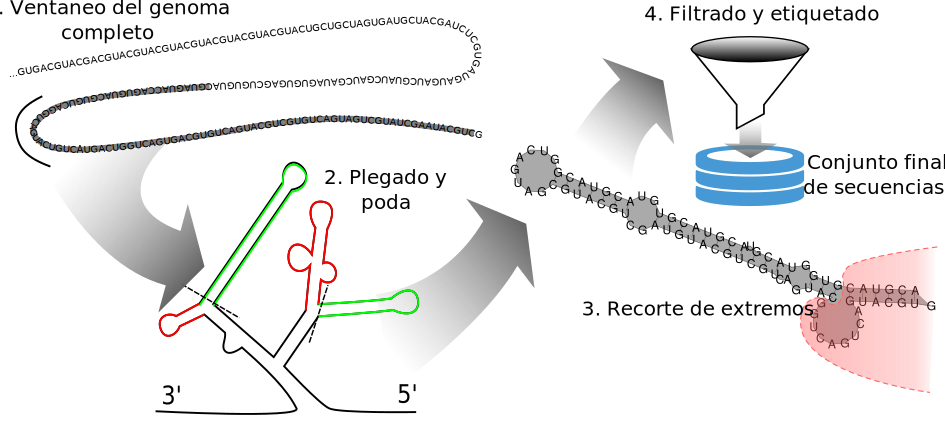
\includepdf[pages=-]{hextractor/hextractor.pdf}
	\chapter{miRNAfe: a comprehensive tool for feature extraction in microRNA prediction}
	\label{sec:mirnafe}
	\includepdf[pages=-]{mirnafe/mirnafe.pdf}
	\includepdf[pages=-,angle=90]{mirnafe/supplementary_material.pdf}
	\chapter{Genome-wide pre-miRNA discovery from few labeled examples}
	\label{sec:mirnass}
	\includepdf[pages=-]{mirnass/mirnass.pdf}
	\includepdf[pages=-]{mirnass/supplementary_material.pdf}
\end{appendices}

\newpage
\thispagestyle{empty}

\noindent \textbf{\Large Doctorado en Ingeniería}\\
\noindent\textbf{\large Mención en Inteligencia Computacional, Señales y Sistemas}\\

\vspace{1cm}

\noindent\textrm{\large Título de la obra:}\\[0.2 cm]
\noindent\textbf{\Large
Nuevo enfoque de aprendizaje\\[0.1 cm]
semi-supervisado para la identificación\\[0.1 cm]
de secuencias en biobinformática}\\

\vspace{1cm}

\noindent\textrm{\large Autor: Cristian Ariel Yones}\\[0.6 cm]
\noindent\textrm{\large Lugar: Santa Fe, Argentina}\\[0.6 cm]
\noindent\textrm{\large Palabras Claves: }\\[0.6 cm]
\noindent\textrm{\large
aprendizaje maquinal, aprendizaje semi-supervisado, \\ predicción de microRNA, genoma completo.}


\end{document}
